%%%%%%%%%%%%%%%%%%%%%%%%%%%%%%%%%%%%%%%%%
% Masters/Doctoral Thesis
% LaTeX Template
% Version 2.5 (27/8/17)
%
% This template was downloaded from:
% http://www.LaTeXTemplates.com
%
% Version 2.x major modifications by:
% Vel (vel@latextemplates.com)
%
% This template is based on a template by:
% Steve Gunn (http://users.ecs.soton.ac.uk/srg/softwaretools/document/templates/)
% Sunil Patel (http://www.sunilpatel.co.uk/thesis-template/)
%
% Template license:
% CC BY-NC-SA 3.0 (http://creativecommons.org/licenses/by-nc-sa/3.0/)
%
%%%%%%%%%%%%%%%%%%%%%%%%%%%%%%%%%%%%%%%%%

%----------------------------------------------------------------------------------------
%	PACKAGES AND OTHER DOCUMENT CONFIGURATIONS
%----------------------------------------------------------------------------------------

\documentclass[
11pt, % The default document font size, options: 10pt, 11pt, 12pt
oneside, % Two side (alternating margins) for binding by default, uncomment to switch to one side
english, % ngerman for German
singlespacing, % Single line spacing, alternatives: onehalfspacing or doublespacing
%draft, % Uncomment to enable draft mode (no pictures, no links, overfull hboxes indicated)
%nolistspacing, % If the document is onehalfspacing or doublespacing, uncomment this to set spacing in lists to single
%liststotoc, % Uncomment to add the list of figures/tables/etc to the table of contents
%toctotoc, % Uncomment to add the main table of contents to the table of contents
%parskip, % Uncomment to add space between paragraphs
%nohyperref, % Uncomment to not load the hyperref package
headsepline, % Uncomment to get a line under the header
%chapterinoneline, % Uncomment to place the chapter title next to the number on one line
%consistentlayout, % Uncomment to change the layout of the declaration, abstract and acknowledgements pages to match the default layout
]{MastersDoctoralThesis} % The class file specifying the document structure

\usepackage[utf8]{inputenc} % Required for inputting international characters
\usepackage[T1]{fontenc} % Output font encoding for international characters

\usepackage{mathpazo} % Use the Palatino font by default

\usepackage[backend=biber,style=numeric,natbib=true]{biblatex} % Use the bibtex backend with the authoryear citation style (which resembles APA)

\addbibresource{example.bib} % The filename of the bibliography


\usepackage{color}
\usepackage{xcolor}
\usepackage{soul}
\definecolor{mGreen}{rgb}{0,0.6,0}
\definecolor{mGray}{rgb}{0.5,0.5,0.5}
\definecolor{mPurple}{rgb}{0.58,0,0.82}
\definecolor{backgroundColour}{rgb}{0.95,0.95,0.92}

\definecolor{Light}{gray}{.90}
\sethlcolor{Light}


\usepackage[autostyle=true]{csquotes} % Required to generate language-dependent quotes in the bibliography


\usepackage{listings}

\lstdefinestyle{CStyle}{
    backgroundcolor=\color{backgroundColour},
    commentstyle=\color{mGreen},
    keywordstyle=\color{magenta},
    numberstyle=\tiny\color{mGray},
    stringstyle=\color{mPurple},
    basicstyle=\scriptsize,
    %basicstyle=\tiny,
    breakatwhitespace=false,
    breaklines=true,
    captionpos=t,
    keepspaces=true,
    numbers=left,
    numbersep=5pt,
    showspaces=false,
    showstringspaces=false,
    showtabs=false,
    tabsize=2,
    language=C
}

\lstdefinestyle{customasm}{
  belowcaptionskip=1\baselineskip,
  frame=L,
  xleftmargin=\parindent,
  language=[x86masm]Assembler,
  basicstyle=\footnotesize\ttfamily,
  commentstyle=\itshape\color{purple!40!black},
}

\usepackage{placeins}

\usepackage{parskip}

\usepackage{amsmath}
%----------------------------------------------------------------------------------------
%	MARGIN SETTINGS
%----------------------------------------------------------------------------------------

\geometry{
	paper=a4paper, % Change to letterpaper for US letter
	inner=2.5cm, % Inner margin
	outer=3.8cm, % Outer margin
	bindingoffset=.5cm, % Binding offset
	top=1.5cm, % Top margin
	bottom=1.5cm, % Bottom margin
	%showframe, % Uncomment to show how the type block is set on the page
}

%----------------------------------------------------------------------------------------
%	THESIS INFORMATION
%----------------------------------------------------------------------------------------

\thesistitle{End-of-Course Internship Report} % Your thesis title, this is used in the title and abstract, print it elsewhere with \ttitle
\supervisor{Filip \textsc{Novotny}} % Your supervisor's name, this is used in the title page, print it elsewhere with \supname
\examiner{} % Your examiner's name, this is not currently used anywhere in the template, print it elsewhere with \examname
\degree{Engineer} % Your degree name, this is used in the title page and abstract, print it elsewhere with \degreename
\author{Simon \textsc{Bataille}} % Your name, this is used in the title page and abstract, print it elsewhere with \authorname
\addresses{} % Your address, this is not currently used anywhere in the template, print it elsewhere with \addressname

\subject{Embedded Systems} % Your subject area, this is not currently used anywhere in the template, print it elsewhere with \subjectname
\keywords{} % Keywords for your thesis, this is not currently used anywhere in the template, print it elsewhere with \keywordnames
\university{\href{http://www.unicaen.fr}{UNIVERSITY CAEN NORMANDIE}} % Your university's name and URL, this is used in the title page and abstract, print it elsewhere with \univname
\department{\href{http://esix.unicaen.fr/}{ESIX NORMANDIE}} % Your department's name and URL, this is used in the title page and abstract, print it elsewhere with \deptname
\group{\href{https://ibubble.camera}{\textsc{Notilo+}}} % Your research group's name and URL, this is used in the title page, print it elsewhere with \groupname
\faculty{\href{http://esix.unicaen.fr/formations/ingenieur-en-mecatronique-et-systemes-nomades/}{Mechatronics \& Nomad Systems}} % Your faculty's name and URL, this is used in the title page and abstract, print it elsewhere with \facname

\AtBeginDocument{
\hypersetup{pdftitle=\ttitle} % Set the PDF's title to your title
\hypersetup{pdfauthor=\authorname} % Set the PDF's author to your name
\hypersetup{pdfkeywords=\keywordnames} % Set the PDF's keywords to your keywords
}

\begin{document}

\frontmatter % Use roman page numbering style (i, ii, iii, iv...) for the pre-content pages

\pagestyle{plain} % Default to the plain heading style until the thesis style is called for the body content

%----------------------------------------------------------------------------------------
%	TITLE PAGE
%----------------------------------------------------------------------------------------

\begin{titlepage}
\begin{center}

\vspace*{.06\textheight}
{\scshape\LARGE \univname\par}\vspace{1.5cm} % University name
\textsc{\Large Engineering Degree}\\[0.5cm] % Thesis type

\HRule \\[0.4cm] % Horizontal line
{\huge \bfseries \ttitle\par}\vspace{0.4cm} % Thesis title
\HRule \\[1.5cm] % Horizontal line

\begin{minipage}[t]{0.4\textwidth}
\begin{flushleft} \large
\emph{Author:}\\
\href{}{\authorname} % Author name - remove the \href bracket to remove the link
\end{flushleft}
\end{minipage}
\begin{minipage}[t]{0.4\textwidth}
\begin{flushright} \large
\emph{Supervisor:} \\
\href{}{\supname} % Supervisor name - remove the \href bracket to remove the link
\end{flushright}
\end{minipage}\\[3cm]

\vfill

\large \textit{A report submitted in fulfillment of the requirements\\ for the degree of \degreename}\\[0.3cm] % University requirement text
\textit{in the}\\[0.4cm]
\groupname\\\deptname\\[2cm] % Research group name and department name

\vfill


\begin{figure}[t]
  \centering
  \begin{minipage}[t]{0.45\textwidth}
    %
\includegraphics[width=\textwidth]{logoEsix}
	  
\includegraphics[scale=0.4]{logoEsix}
  \end{minipage}
  \hfill
  \begin{minipage}[t]{0.3\textwidth}
    %
\includegraphics[width=\textwidth]{logoNotilo}
	  
\includegraphics[scale=1.0]{logoNotilo}
  \end{minipage}
\end{figure}


{\large \today}\\[4cm] % Date

\vfill
\end{center}
\end{titlepage}

%----------------------------------------------------------------------------------------
%	DECLARATION PAGE
%----------------------------------------------------------------------------------------

%\begin{declaration}
%\addchaptertocentry{\authorshipname} % Add the declaration to the table of contents
%\noindent I, \authorname, declare that this thesis titled, \enquote{\ttitle} and the work presented in it are my own. I confirm that:
%
%\begin{itemize}
%\item This work was done wholly or mainly while in candidature for a research degree at this University.
%\item Where any part of this thesis has previously been submitted for a degree or any other qualification at this University or any other institution, this has been clearly stated.
%\item Where I have consulted the published work of others, this is always clearly attributed.
%\item Where I have quoted from the work of others, the source is always given. With the exception of such quotations, this thesis is entirely my own work.
%\item I have acknowledged all main sources of help.
%\item Where the thesis is based on work done by myself jointly with others, I have made clear exactly what was done by others and what I have contributed myself.\\
%\end{itemize}
%
%\noindent Signed:\\
%\rule[0.5em]{25em}{0.5pt} % This prints a line for the signature
%
%\noindent Date:\\
%\rule[0.5em]{25em}{0.5pt} % This prints a line to write the date
%\end{declaration}
%
%\cleardoublepage

%----------------------------------------------------------------------------------------
%	QUOTATION PAGE
%----------------------------------------------------------------------------------------

\vspace*{0.2\textheight}

\noindent\enquote{\itshape Thanks to my solid academic training, today I can write hundreds of words on virtually any topic without possessing a shred of information, which is how I got a good job in journalism.}\bigbreak

\hfill Dave Barry

%----------------------------------------------------------------------------------------
%	ABSTRACT PAGE
%----------------------------------------------------------------------------------------

\begin{abstract}
\addchaptertocentry{\abstractname} % Add the abstract to the table of contents
The Thesis Abstract is written here (and usually kept to just this page). The page is kept centered vertically so can expand into the blank space above the title too\ldots
\end{abstract}

%----------------------------------------------------------------------------------------
%	ACKNOWLEDGEMENTS
%----------------------------------------------------------------------------------------

\begin{acknowledgements}
\addchaptertocentry{\acknowledgementname} % Add the acknowledgements to the table of contents
The acknowledgments and the people to thank go here, don't forget to include your project advisor\ldots
\end{acknowledgements}

%----------------------------------------------------------------------------------------
%	LIST OF CONTENTS/FIGURES/TABLES PAGES
%----------------------------------------------------------------------------------------

\tableofcontents % Prints the main table of contents

\listoffigures % Prints the list of figures

\listoftables % Prints the list of tables

%----------------------------------------------------------------------------------------
%	ABBREVIATIONS
%----------------------------------------------------------------------------------------

\begin{abbreviations}{ll} % Include a list of abbreviations (a table of two columns)

\textbf{LAH} & \textbf{L}ist \textbf{A}bbreviations \textbf{H}ere\\
\textbf{WSF} & \textbf{W}hat (it) \textbf{S}tands \textbf{F}or\\
\textbf{API} & \textbf{A}pplication \textbf{P}rogramming \textbf{I}nterface\\
\textbf{AI} & \textbf{A}rtificial \textbf{I}ntelligence\\
\textbf{BtB} & \textbf{B}usiness \textbf{t}o \textbf{B}usiness\\
\textbf{BtC} & \textbf{B}usiness \textbf{t}o \textbf{C}ustomers\\
\textbf{CMT} & \textbf{C}lustering of Static-Adaptative Correspondences for Defor\textbf{M}able Object \textbf{T}racking\\
\textbf{CPU} & \textbf{C}entral \textbf{P}rocessing \textbf{U}nit\\
\textbf{DMA} & \textbf{D}irect \textbf{M}emory \textbf{A}ccess\\
\textbf{fps} & \textbf{f}rames \textbf{p}er \textbf{s}second\\
\textbf{GPU} & \textbf{G}raphics \textbf{P}rocessing \textbf{U}nit\\
\textbf{SIMD} & \textbf{S}ingle \textbf{I}nput \textbf{M}ultiple \textbf{D}ata\\
\textbf{SoC} & \textbf{S}ystem \textbf{o}n \textbf{C}hip\\
\textbf{QPU} & \textbf{Q}uad \textbf{P}rocessor \textbf{U}nit\\
\textbf{VPM} & \textbf{V}ertex \textbf{P}ipe \textbf{M}emory\\
%Consensus-based Tracking and Matching of Keypoints for Object Tracking
\end{abbreviations}

%----------------------------------------------------------------------------------------
%	PHYSICAL CONSTANTS/OTHER DEFINITIONS
%----------------------------------------------------------------------------------------

\begin{constants}{lr@{${}={}$}l} % The list of physical constants is a three column table

% The \SI{}{} command is provided by the siunitx package, see its documentation for instructions on how to use it

Speed of Light & $c_{0}$ & \SI{2.99792458e8}{\meter\per\second} (exact)\\
%Constant Name & $Symbol$ & $Constant Value$ with units\\

\end{constants}

%----------------------------------------------------------------------------------------
%	SYMBOLS
%----------------------------------------------------------------------------------------

\begin{symbols}{lll} % Include a list of Symbols (a three column table)

$a$ & distance & \si{\meter} \\
$P$ & power & \si{\watt} (\si{\joule\per\second}) \\
%Symbol & Name & Unit \\

\addlinespace % Gap to separate the Roman symbols from the Greek

$\omega$ & angular frequency & \si{\radian} \\

\end{symbols}

%----------------------------------------------------------------------------------------
%	DEDICATION
%----------------------------------------------------------------------------------------

\dedicatory{For/Dedicated to/To my\ldots}

%----------------------------------------------------------------------------------------
%	THESIS CONTENT - CHAPTERS
%----------------------------------------------------------------------------------------

\mainmatter % Begin numeric (1,2,3...) page numbering

\pagestyle{thesis} % Return the page headers back to the "thesis" style

% Include the chapters of the thesis as separate files from the Chapters folder
% Uncomment the lines as you write the chapters

% Introduction

\chapter{Introduction} % Main chapter title

\label{Introduction} % For referencing the chapter elsewhere, use \ref{Introduction}

%----------------------------------------------------------------------------------------

% Define some commands to keep the formatting separated from the content
\newcommand{\keyword}[1]{\textbf{#1}}
\newcommand{\tabhead}[1]{\textbf{#1}}
%\newcommand{\code}[1]{\texttt{#1}}
\newcommand{\code}[1]{\texttt{\hl{#1}}}
\newcommand{\file}[1]{\texttt{\bfseries#1}}
\newcommand{\option}[1]{\texttt{\itshape#1}}
\newcommand{\iBubble}{\textsc{iBubble}}
\newcommand{\rasp}{\textsc{Raspberry Pi}}
\newcommand{\vc}{\textsc{VideoCore iv 3D}}
\newcommand{\cpu}{\textsc{arm cpu}}
\newcommand{\bcm}{\textsc{bcm2837}}
\newcommand{\qpu}{\textsc{qpu}}
\newcommand{\flow}{\textsc{optical flow}}
\newcommand{\feat}{\textsc{feature}}
\newcommand{\api}{\textsc{api}}
\newcommand{\ram}{\textsc{shared ram}}
\newcommand{\mail}{\textsc{mailbox}}
\newcommand{\uni}{\textsc{uniform}}

%----------------------------------------------------------------------------------------

\section{\textsc{Notilo+} \& \textsc{iBubble}}

\footnote{\groupname{}: \url{https://ibubble.camera/}}\groupname{} is a young and innovative start-up based in Lyon. It was created in 2016 by Nicolas \textsc{Gambini} and Benjamin \textsc{Valtin} and early funded through crowd-funding during the 2016 year.

Currently about 20 people are working at \groupname{}. The company is divided into two parts: a business and commercial section and a technical section.

This technical section consists of an hardware-oriented team with mechanical and electronics engineers, an embedded sofware team of low-level developers and a vision team that I have joined. This team is composed of Filip the Computer Vision lead and my personnal supervisor, Loic a Computer Vision engineer, Nima a Robotics engineer and Camille a Computer Vision trainee.

The objective of \groupname{} is to develop and sell an \emph{autonomous} and \emph{wireless} underwater drone called \iBubble.

\begin{figure}[h]
\centering
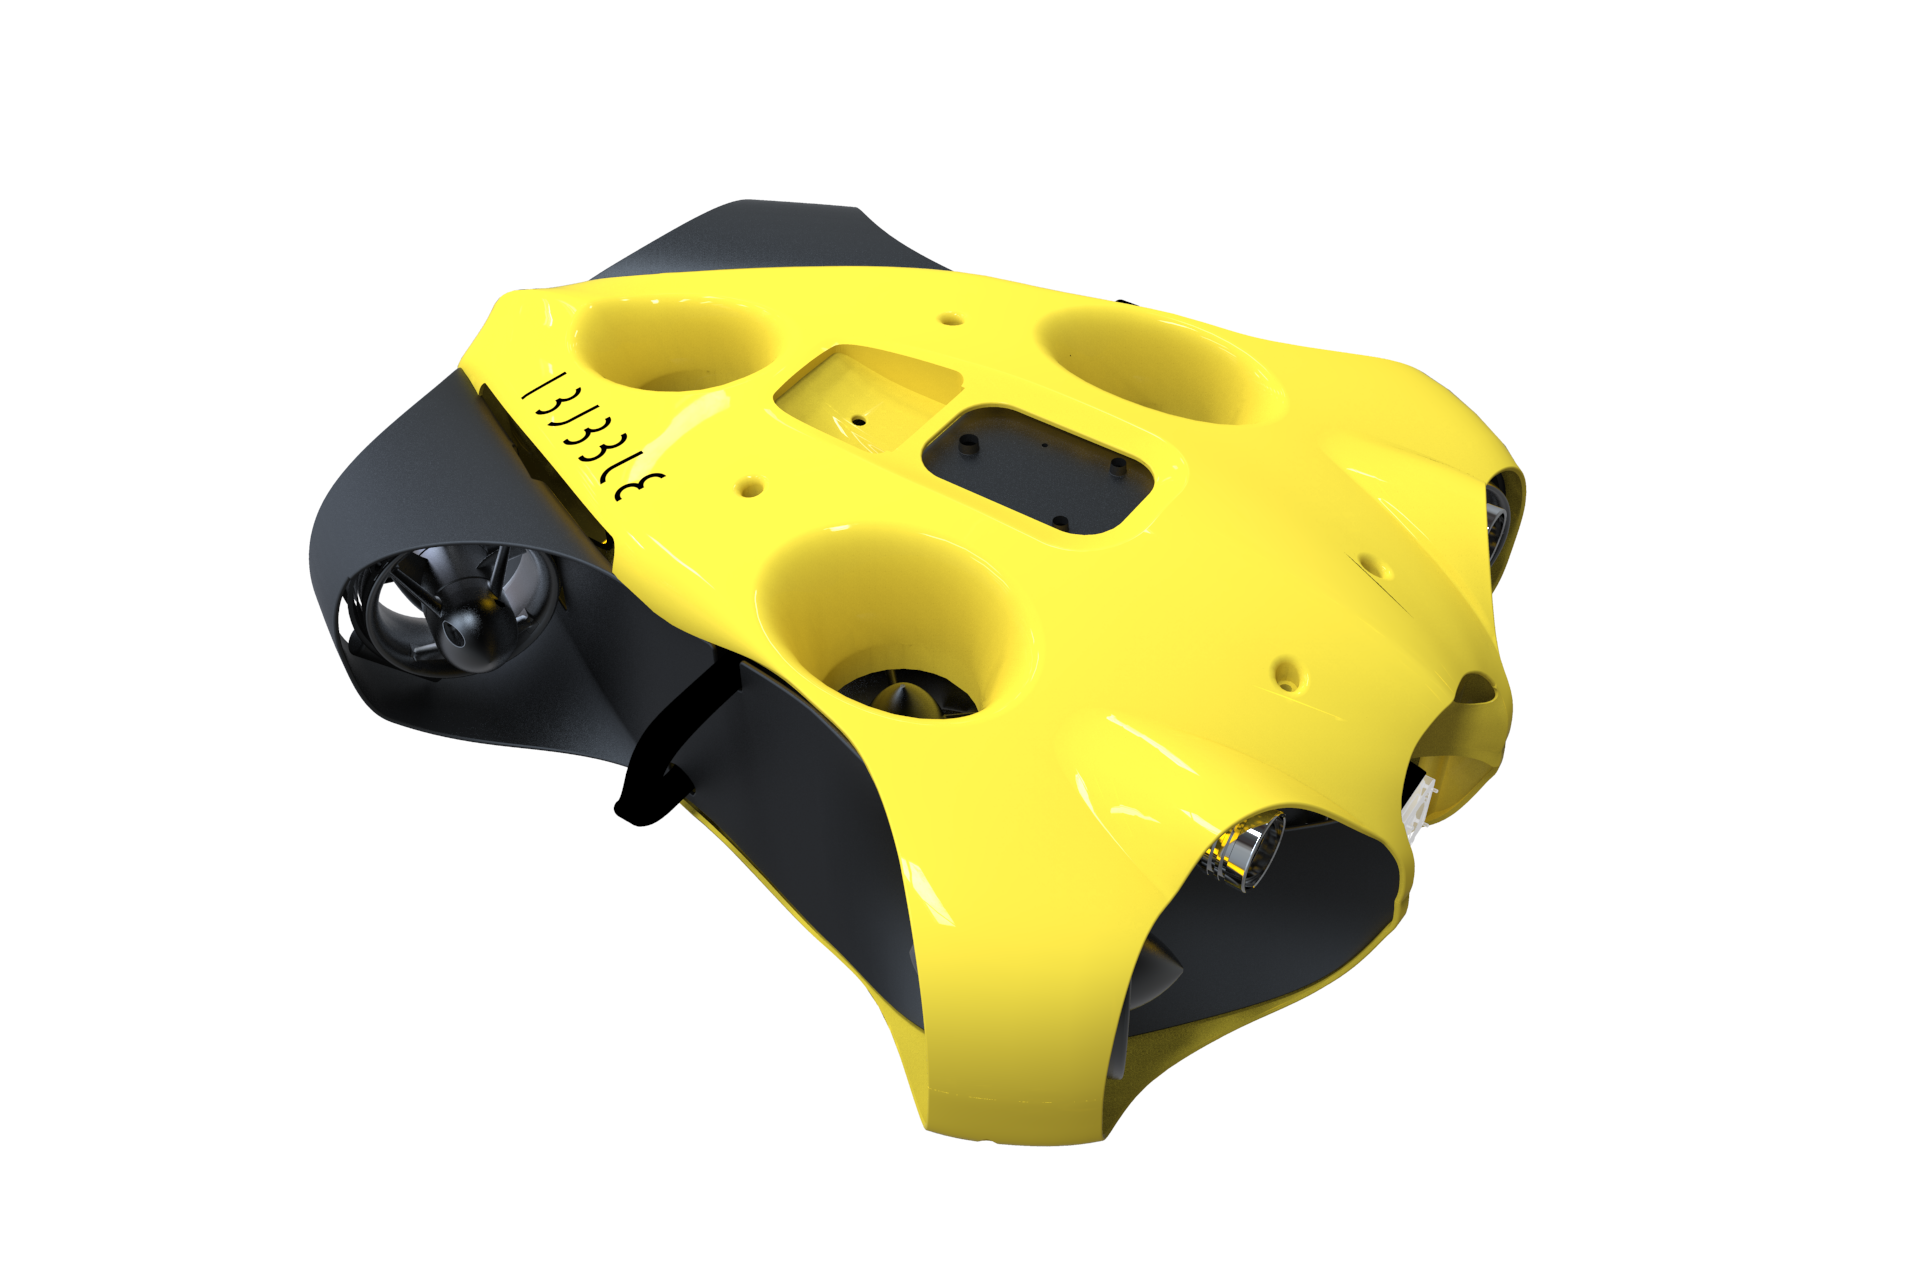
\includegraphics[width=0.4\textwidth]{iBubble3}
\caption{\iBubble{} drone}
\end{figure}


\iBubble{} is designed to replace cameraman divers. It can \emph{autonomously} follow a diver and capture footages from the diving session without any action from the user. The targeted \keyword{BtC} audience are for instance professional divers, diving centers, free-divers or resorts.

A live video feedback is also available on \iBubble. In this mode, a cable link between the drone and the user enables the video feedback on a smartphone and users can explore unknown spots before diving.\\


In addition to this \keyword{BtC} sector, \iBubble{} is suitable for a large range of \keyword{BtB} applications. Indeed, it can integrate multiple specific feat{}s for companies that have real needs in underwater inspection such as dam, harbor or simply ship's hull. Thanks to its \emph{autonomous} ability, it will be able to verify the good shape of a concrete wall for example and provides videos of its inspection.

%----------------------------------------------------------------------------------------

\section{Autonomous Tracking System}

As I said in the previous section, \iBubble's main feature is to follow \emph{autonomously} a diver to film the diving session. The diver can only choose one of the drone's available scenarii such as \emph{follow me}, \emph{circle me}, \emph{follow me side} etc. At any time the diver, or someone else is controlling the drone with a joystick. Because of the countless difficulties raised by underwater environments (no GPS, no Wi-Fi etc.), \emph{autonomously} follow a diver is a high technical challenge. To achieve this goal, \iBubble{} uses two technologies: \emph{acoustic} and \emph{vision} location.

The whole \iBubble's \emph{Autonomous Tracking System} -- acoustic and vision -- is implemented in a project called \keyword{NotiloTracker}.

\subsection{Acoustic System}

The diver is outfitted with a remote control that is an \emph{acoustic} emitter sending ultrasound pulses. \iBubble{} detects those pulses thanks to five \emph{acoustic} receivers and locates approximately the diver. This \emph{acoustic} positioning system is not very accurate because of the heavily perturbated underwater environment. As a consequence a \emph{vision} system is used to locate the diver in parallel.


\subsection{Vision System}

\label{Vision} % For referencing the chapter elsewhere, use \ref{Vision}

\iBubble{} has two cameras at his disposal: one to record the diving session (generally a \emph{GoPro} camera) and another one to capture frames used in the computer vision part. This camera is generally a cheaper camera with a low resolution. When \iBubble{} is opposite the diver it can detect the position more precisely thanks to several algorithms running on the embedded board.

The vision system is globally composed of two parts: a \emph{machine learning detector} to lock the position of the diver and a \emph{tracker} to follow him between two frames of the video. The bulk of complexity is to compute the \flow{} for the \emph{tracking} algorithm and in Forward Propagation of a Convolutional Neural Network for the \emph{detector} algorithm.

%----------------------------------------------------------------------------------------

\section{Internship}

\subsection{Problematics}

The vision algorithms mentionned in~\ref{Vision} are well-known and can be parallelized very efficiently on \keyword{GPU}s to improve compute speed. Therefore there are a lot of implementations on \keyword{GPU}s of these algorithms especially with the growth of \emph{Nvidia's CUDA GPGPU cores} on embedded chip (for instance the Jetson TX2 board).

However, \groupname{} chose \rasp\footnote{Raspberry Pi: \url{https://www.raspberrypi.org/}} as the central embedded computer for \iBubble. Indeed, this board is far less expensive than \emph{CUDA} systems, reasonably powerful and very well-documented with a huge community of developers.\par

The \keyword{SoC} used in the \rasp{} is a \keyword{\textsc{Broadcom}} \bcm{}\footnote{BCM2837: \url{https://www.raspberrypi.org/app/uploads/2012/02/BCM2835-ARM-Peripherals}} fitted with:
\begin{itemize}
\item \keyword{CPU} -- \keyword{ARM Cortex A53} (ARMv8) cluster
\item \keyword{GPU} -- \vc{}
\end{itemize}

Furthermore, the current vision system (\emph{detector \& tracker}~\ref{Vision}) uses state-of-the-art algorithm \keyword{CMT}\footnote{CMT algorithm: \url{https://www.gnebehay.com/cmt/}}, developed with \keyword{OpenCV}\footnote{OpenCV: \url{https://opencv.org/}} the main library used in Computer Vision.

The main issue is that the \bcm{} is not designed with a \emph{CUDA} architecture and there is no reliable implementation of the algorithms on the \rasp. As a consequence, the \vc{} can't be used and the whole \emph{tracking system} is running only on the \rasp's \keyword{CPU}, resulting in slow computing time and poor performances. Since all the vision system will be integrated on the \rasp, the difficulty is to achieve correct quality with a real-time processing on a such device.

To meet these objectives, \groupname{} have decided to developp its own implementation of those algorithms using an homemade \keyword{API} for the \vc. This is the subject of my internship.


\subsection{Subject}

From low-level programming to image processing and numerical analysis, this subject covers a wide range of fields. Therefore, the internship work has been split into two internships:

\begin{itemize}
\item \keyword{API} for the \keyword{GPU}: with my background on embedded systems, I was focused on the \vc{} programming
\item Algorithms Implementation: another intern, Camille \textsc{Farineau}, was focused on the \keyword{tracking \& detctor} algorithms implementation
\end{itemize}


\subsubsection{Algorithms Implementation}

Camille's job was to work on:

\begin{itemize}
	\item \emph{Machine Learning} algorithm for the \emph{detector}
	\item \flow{} computation -- part of \keyword{CMT} algorithm -- for the \emph{tracker}
\end{itemize}

Indeed, before implementing these algorithms on the \vc, it was crucial that \groupname{} has its own implementation of them. Currently all the vision system is coded in \keyword{C++} and uses libraries such as \emph{OpenCV}. Camille had to work on these algorithms with the technologies, libraries, frameworks that fit the best the problem, namely processing parts of these algorithms on the \vc{} in order to release some \keyword{CPU} ressources.

In a first time he has to study and understand the popular implementations of the \flow{} algorithms, create a state-of-the-art document of these algorithms. Then he suggests an optimized implementation for the chosen method. This implementation must be highly parallelizable in order to use the \vc. At this stage, wa have to communicate together so that I understand how the \vc{} can be helpful for the implementation of the \flow{} algorithm.

Next this algorithm needs to be test in simulation and real conditions on the \rasp. This step is fundamental to estimate the gain and loss in quality and computing time compared to the current solution. Finally the last part is to implement it on the drone system and test the whole vision system with the new \flow{} algorithm.


\subsubsection{API for the \textsc{VideoCore IV 3D GPU}}

Personnaly I had to study and understand the \vc{}. The goal was to create an homemade \keyword{API} accessible from a high-level language such as \keyword{C++}. This \keyword{API} was to provide basic functions to run computations of the \flow{} algorithm on the \vc{} in order to achieve a real time performance and relieve the \keyword{CPU}.

Due to the growing popularity of the \rasp{}, \keyword{\textsc{Broadcom}} released an official \vc{} architecture reference guide\footnote{\vc{} Documentation: \url{https://docs.broadcom.com/docs/12358545}}, but without any official \keyword{API}.

As a conseqence, the main questions for me was to study the architecture and understand how to use the \vc{}, then understand the \flow{} algorithm and implement an optimized and parallelized version running on the \vc{}.

Camille and I worked in parallel but we had to coordinate ourselves in order to develop the dedicated functions. Camille had to specify the needs for the \flow{} algorithm (what kind of computations such as a convolution, gradient or interpolation functions etc.) and I have to adapt the \keyword{API} to integrate these functions on a program running of the \vc.

%----------------------------------------------------------------------------------------

% Chapter 2

\chapter{Internship work} % Main chapter title

\label{Chapter2} % For referencing the chapter elsewhere, use \ref{Chapter2}

%----------------------------------------------------------------------------------------

% Define some commands to keep the formatting separated from the content
%\newcommand{\keyword}[1]{\textbf{#1}}
%\newcommand{\tabhead}[1]{\textbf{#1}}
%\newcommand{\code}[1]{\texttt{#1}}
%\newcommand{\file}[1]{\texttt{\bfseries#1}}
%\newcommand{\option}[1]{\texttt{\itshape#1}}
%\newcommand{\iBubble}{\textcolor{mdtRed}{\textsc{iBubble}}}
%\newcommand{\rasp}{\textcolor{mdtRed}{\textsc{Raspberry Pi}}}
%\newcommand{\vc}{\textcolor{mdtRed}{\textsc{VideoCore IV 3D}}}
%\newcommand{\cpu}{\textcolor{mdtRed}{\textsc{ARM CPU}}}
%\newcommand{\bcm}{\textcolor{mdtRed}{\textsc{BCM2837}}}
%\newcommand{\qpu}{\textcolor{mdtRed}{\textsc{QPU}}}
%\newcommand{\code}[1]{\texttt{\hl{#1}}}
\definecolor{mGreen}{rgb}{0,0.6,0}
\definecolor{mGray}{rgb}{0.5,0.5,0.5}
\definecolor{mPurple}{rgb}{0.58,0,0.82}
\definecolor{backgroundColour}{rgb}{0.95,0.95,0.92}

%----------------------------------------------------------------------------------------

\section{State of the Art}

When arriving at \groupname{}, my first task was to write a \emph{State-of-the-Art} report about the \vc{}. The goal was to list interesting projects using this \keyword{GPU} and know what was possible to do with it.

I spent my first two weeks surfing on the internet to gather every information I found about \vc. I wrote a report containing general information and every accurate project for the rest of my internship.

Finally I had a meeting with \supname{} where I explained to him which direction I wanted to explore. We decided that I should start with a \emph{\enquote{helloworld}} program that made me understand the basics of the \vc{} and start developping on a \rasp.

%----------------------------------------------------------------------------------------

\section{Raspberry Pi Playground}

\emph{Raspberry Pi Playground} \parencite{refRpiPlayground} is the first project I focused on to better understand the \vc. It is associated with a \enquote{\file{github}} repository: \url{//github.com/elorimer/rpi-playground}

It is the most important project I studied during my internship because it contains a \enquote{\file{helloworld}} program that helped me to understand the preliminary basis of the \vc{} architecture and above all, how to use this \keyword{GPU}.

I followed every step of this project permanantly reading the \vc{} documention \parencite{refVC}. I detail this program because all the rest of my internship is based on it.

\subsection{GPU Programming}
\label{concepts}
Before describing what the \file{helloworld} project does, I will highlight some \keyword{key points} in \vc{} programming that I understood with \parencite{refRpiPlayground}:

\begin{itemize}
	\item GPU is a CPU peripheral
	\item GPU and CPU share the same RAM memory
\end{itemize}

-- \keyword{First key thing} to understand is that a \keyword{GPU} is driven by a host \keyword{CPU}. In the case of \bcm, the \vc{} is driven by an \cpu{}.

-- \keyword{Second key thing} is that they share the same \keyword{RAM} memory.

These are really two crucial \keyword{concepts} to keep in mind for the rest of the report. It took me time to understand them although it is the heart of \vc{} programming.

\vspace{5mm}
Thus to run \code{code} on \keyword{GPU}, the host \keyword{CPU}:
\begin{itemize}
	\item \code{define} \& \code{map} a \ram{} memory space between both processors
	\item \code{send} instructions and data using \emph{VC CPU Bus Addresses}
	\item \code{get back} results from \keyword{GPU} also using \emph{VC CPU Bus Addresses}
\end{itemize}

Appendice~\ref{AppendixB} taken from the \bcm{} documentation \parencite{refBCM} shows these different address spaces.



\subsection{\file{helloworld} Program}

As a consequence of \ref{concepts}, in the case of \keyword{GPU} programing, a \file{helloworld} is not a trivial exercice because a lot of parts are involved. To run \code{code} on \vc, we must write a \cpu{} program \option{in c language} that will:
\begin{itemize}
	\item initialize the GPU
	\item map \ram{} memory space
	\item configure parameters
	\item send data and code to the GPU
	\item get back resutls
\end{itemize}
\vspace{5 mm}

Within the \file{rpi-playground} project, \file{helloworld} program will:

\begin{itemize}
	\item initialize the \vc
	\item map the \ram{} memory space between the \vc{} and the \cpu
	\item transfer a single input value - \keyword{100} - from \cpu{} to \vc
	\item use the \vc{} to add constant  - \keyword{0x1234} - to this input value
	\item get back the result from \vc{} to \cpu
\end{itemize}

\newpage
\subsubsection{Run helloworld and see its output}

To execute \file{helloworld}, we run \code{sudo ./helloworld helloworld.bin 100}.

\code{./helloworld} is responsible for mapping memory, initialize \keyword{GPU}, get back results and sends two arguments to the \keyword{GPU}:
\begin{itemize}
	\item \keyword{100} -- the input value
	\item \file{helloworld.bin} -- \code{code-to-execute} by \vc{} that contains \keyword{0x1234} value
\end{itemize}

Finally, program adds \keyword{100} to \keyword{0x1234} and produces the following output:

\lstset{style=CStyle,caption={\file{helloworld} output},captionpos=t}
\begin{lstlisting}
Loaded 80 bytes of code from helloworld.bin ...
QPU enabled.
Uniform value = 100
QPU 0, word 0: 0x00001298
QPU 0, word 1: 0x00001298
QPU 0, word 2: 0x00001298
QPU 0, word 3: 0x00001298
QPU 0, word 4: 0x00001298
QPU 0, word 5: 0x00001298
QPU 0, word 6: 0x00001298
QPU 0, word 7: 0x00001298
QPU 0, word 8: 0x00001298
QPU 0, word 9: 0x00001298
QPU 0, word 10: 0x00001298
QPU 0, word 11: 0x00001298
QPU 0, word 12: 0x00001298
QPU 0, word 13: 0x00001298
QPU 0, word 14: 0x00001298
QPU 0, word 15: 0x00001298
Cleaning up.
Done.
\end{lstlisting}


\subsection{\vc{} Overview}



Appendice~\ref{AppendixC} taken from \parencite{refVC} shows an architecture overview of the \vc. \keyword{GPU}'s parts involved in \file{helloworld} program are highlighted with \textcolor{blue}{blue rectangles}:


\begin{itemize}
	\item \keyword{AXI ARB} -- bus that connects \vc{} to \ram{} and \cpu
	\item \keyword{Uniforms Cache (QUC)} -- cache containning \code{variables} transferred from \cpu{} to \vc
	\item \keyword{Icache (QIC)} -- cache containning \code{code-to-execute} transferred from \cpu{} to \vc
	\item \keyword{Quad Processor Unit (QPU)} -- \vc{} internal processor
	\item \keyword{Vertex Pipe Memory (VPM)} -- \vc{} internal memory buffer
	\item \keyword{VPM DMA Writer (VDM)} -- writes DATA from VPM to \ram{}
	\item \keyword{Vertex Cache Manager \& DMA (VCM and VCD)} -- writes DATA from \ram{} to VPM
\end{itemize}
\vspace{5 mm}

\cpu{} and \vc{} communicate through \keyword{AXI ARB} bus. Within \file{helloworld} program, we will use \cpu{} to:
\begin{itemize}
	\item initialize and allocate \ram{} accessible in both \emph{ARM Virtual Adresses} and \emph{VC CPU Bus Adresses} - Appendice~\ref{AppendixB}
	\item transfer \code{variables} to the \keyword{QUC}
	\item transfer \code{code-to-execute} to the \keyword{QIC}
	\item execute \code{code} with \keyword{QPU}
	\item store result into \keyword{VPM}
	\item write back results into \ram{} through \keyword{VDM}
\end{itemize}


\subsubsection{Quad Processor Unit}

\qpu{} is the \vc{} internal processor. It is the \keyword{key component}. Appendice~\ref{AppendixD} taken from \parencite{refVC} shows its pipeline.


\qpu{} is a \keyword{SIMD} vector processor developed by \textsc{Broadcom} with instructions that operate on 16-element vectors of 32-bit integer or floating point values. For example, given two 16-element vectors:\\

\begin{tabular}{cccc|cccc|cccc|cccc}
	10&11&12&13&14&15&16&17&18&19&20&21&22&23&24&25
\end{tabular}

and

\begin{tabular}{cccc|cccc|cccc|cccc}
	20&21&22&23&24&25&26&27&28&29&30&31&32&33&34&35
\end{tabular}\\

The \qpu's \code{integer-add} instruction - Figure~\ref{VCinstructionsFigure} - computes a third vector:

\begin{tabular}{cccc|cccc|cccc|cccc}
	30&32&34&36&38&40&42&44&46&48&50&52&54&56&58&60
\end{tabular}

where each element in the output is the sum of the corresponding two elements in the inputs.\\

Each 16-element vector is comprised of four quads. This is where the name ``Quad Processing Unit'' comes from: a QPU processes one quad per clock cycle, and a QPU instruction takes four consecutive clock cycles to deliver a full 16-element result vector.

\rasp{} contains 12 \qpu{}s in total, each running at 250MHz. That's a max throughput of 750M vector instructions per second (250M cycles divided by 4 cycles-per-instruction times 12 QPUs). Or: 12B operations per second (750M instructions times 16 vector elements). \qpu{} instructions can in some cases deliver two results at a time, so the Pi's QPUs are often advertised at 24 GFLOPS.
\newpage


\subsection{\file{rpi-playground} Architecture}

\begin{figure}[!htbp]
	\centering
	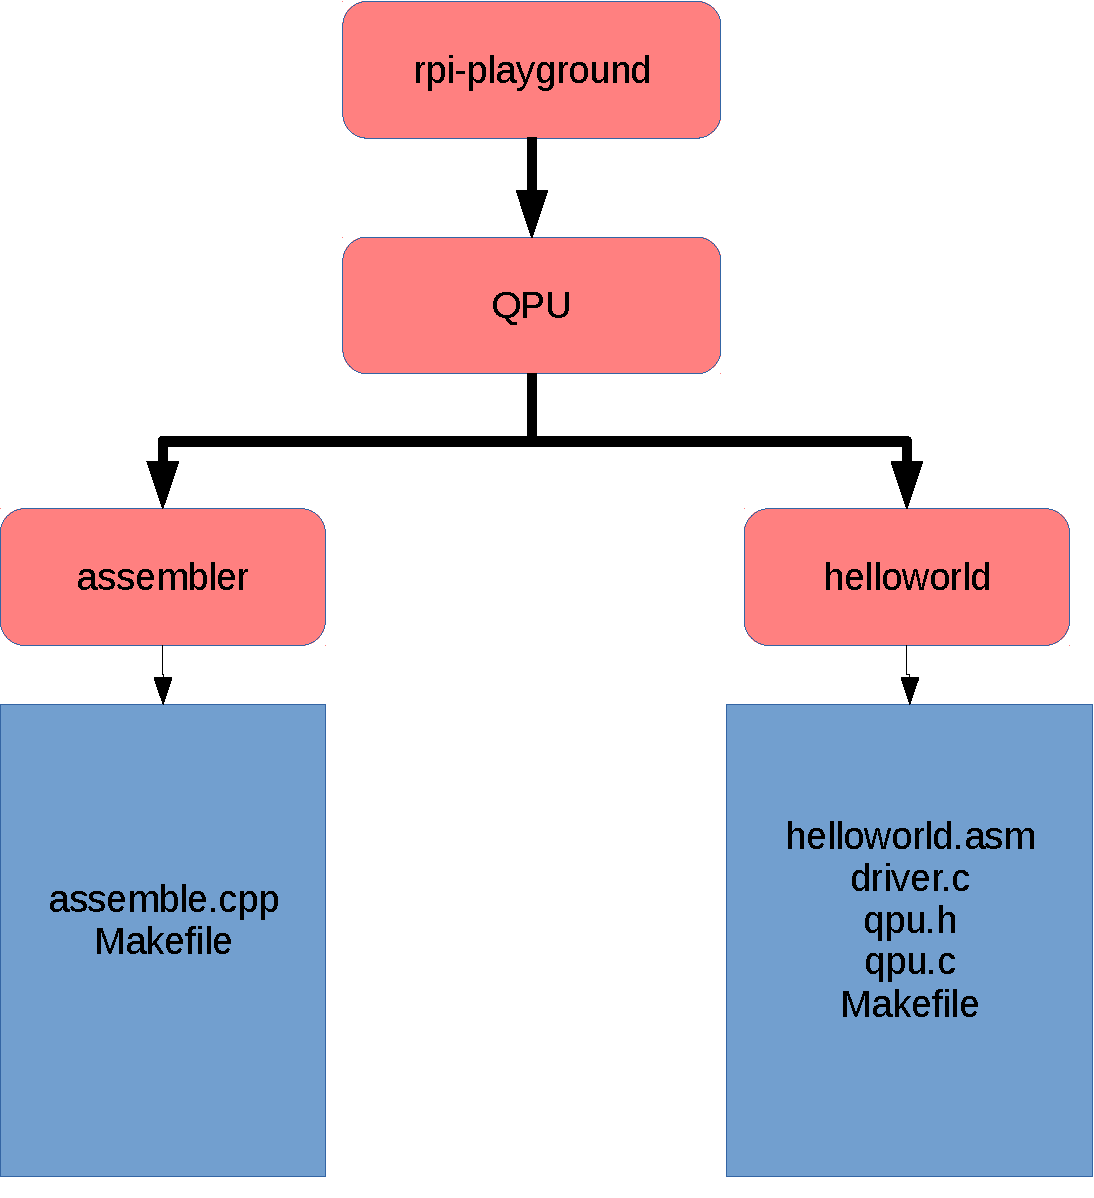
\includegraphics[width=0.4\textwidth,scale=0.2]{rpiPlaygroundArchitecture}
	\caption{\file{rpi-playground} Architecture}
	\label{rpiPlaygroundFigure}
\end{figure}
\FloatBarrier

Figure~\ref{rpiPlaygroundFigure} shows the architecture of the \file{rpi-playground} project once cloned from the \file{github} repository: \code{git clone git@github.com:elorimer/rpi-playground.git}

The project is made of two directories:
\begin{itemize}
\item \keyword{assembler} directory contains:
	\begin{itemize}
		\item \file{assemble.cpp} -- \code{assembly parser} of \vc{} instructions set
	\end{itemize}
\item \keyword{helloworld} directory contains:
	\begin{itemize}
		\item \file{helloworld.asm} -- \code{code-to-execute} on the \vc
		\item \file{driver.c} -- program that \code{drives} the \vc
	\end{itemize}
\end{itemize}


\subsection{\keyword{assembler} directory}


\subsubsection{assemble.cpp}

\file{assemble.cpp} is the \code{assembly parser} written by Eric \textsc{Lorimer}, the author of \file{rpi-playground} project.

This program translates instuctions written in \file{helloworld.asm} - from \file{helloworld} directory figure~\ref{rpiPlaygroundFigure} - into a binary file - \file{helloworld.bin} - that the \vc{} will understand.

Figure~\ref{VCinstructionsFigure} taken from \parencite{refVC} shows the miscellaneous \enquote{\code{add}} operations of the \qpu's instructions set. \vc{} has also \enquote{\code{mul}}, \enquote{\code{load}}, \enquote{\code{branch}} or \enquote{\code{semaphore}} instructions.

\begin{figure}[!htbp]
	\centering
	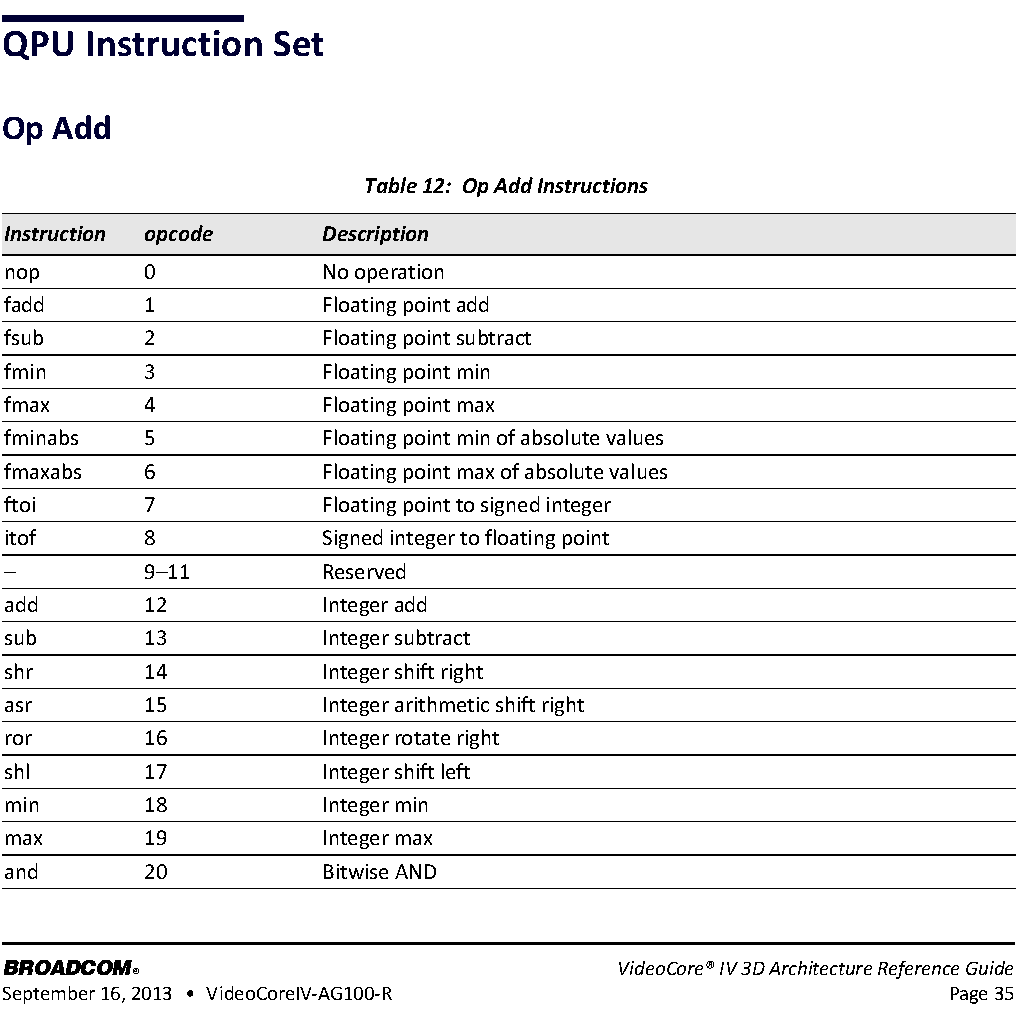
\includegraphics[width=0.6\textwidth]{VCinstructions}
	\caption{Part of \vc{} instructions set}
	\label{VCinstructionsFigure}
\end{figure}
\FloatBarrier
\vspace{5mm}


In \file{assemble.cpp}, these instructions are declared with the following \keyword{C++} code:

\lstset{style=CStyle,caption={Declaration of \code{add} operations in \file{assemble.cpp}},captionpos=t,label=addLabel}
\begin{lstlisting}
static string addOps[] = {
    "nop", "fadd", "fsub", "fmin", "fmax", "fminabs", "fmaxabs",
    "ftoi", "itof", "XXX", "XXX", "XXX", "add", "sub", "shr",
    "asr", "ror", "shl", "min", "max", "and", "or", "xor", "not",
    "clz", "XXX", "XXX", "XXX", "XXX", "XXX", "v8adds", "v8subs" };
\end{lstlisting}


\subsubsection{Makefile}

\lstset{language=make,caption={Makefile from assembler directory},captionpos=t,label=assMakefileLabel}
\begin{lstlisting}
qpu-assembler: assemble.cpp
	g++ -g -o qpu-assembler assemble.cpp
\end{lstlisting}

This \file{Makefile} contains only one instruction. So running the \code{make} command inside the \keyword{assembler} directory generates an \keyword{executable} file: \file{qpu-assembler}.
\vspace{10mm}

Then, this \keyword{executable} is used in the \file{helloworld} directory to generate \file{helloworld.bin}:
\begin{center}
\code{../assembler/qpu-assembler -o helloworld.bin < helloworld.asm}
\end{center}
\newpage

\subsection{helloworld directory}

\subsubsection{qpu.h/qpu.c}

In these files we define \code{BUS\_TO\_PHYS()}, a \code{MACRO} function to convert \emph{VC CPU Bus Addresses} into \emph{ARM Virtual Addresses} - Appendice~\ref{AppendixB}.

Then we use \code{MACROS} to define the \emph{VC CPU Bus Addresses}'s of \vc{} peripherals.

Finally, we declare \code{gpu\_fft\_get\_host\_info()} to get \rasp{} information.

\lstset{style=CStyle,caption={qpu.h}}
\begin{lstlisting}
#define BUS_TO_PHYS(x) ((x)&~0xC0000000)

#define V3D_L2CACTL (0xC00020>>2)
#define V3D_SLCACTL (0xC00024>>2)
#define V3D_SRQPC   (0xC00430>>2)
#define V3D_SRQUA   (0xC00434>>2)
#define V3D_SRQCS   (0xC0043c>>2)
#define V3D_DBCFG   (0xC00e00>>2)
#define V3D_DBQITE  (0xC00e2c>>2)
#define V3D_DBQITC  (0xC00e30>>2)

int gpu_fft_get_host_info(struct GPU_FFT_HOST *info);
\end{lstlisting}


\subsubsection{helloworld.asm}

\file{helloworld.asm} is the \code{code-to-execute} by the \vc. It is written in \option{assembly language} using the \vc{}'s instructions set. Let's explain this \file{file} line by line:\\

\code{\# Load the value we want to add to the input into a register\\ldi ra1, 0x1234}\\
-- First, we load the 32-bit immediate value \emph{0x1234} into \emph{ra1} register.\\
-- This value is replicated 16 ways accross the entire SIMD array of the \emph{QPU 0,0} processor.\\

\code{\# Configure the VPM for writing\\ldi rb49, 0xa0}\\
-- \qpu{} register address map in \parencite{refVC} pages 37-38 shows writting to \emph{rb49} is \code{VPMVCD\_WR\_SETUP}: we configure \keyword{VPM} memory to store results from \emph{QPU 0,0}.\\

\code{\# Add the input value (first uniform - rb32)\\ \# and the register with the hard-coded constant into the VPM.\\add rb48, ra1, rb32; nop}\\
-- \emph{rb48} is the register to write into, in order to write results from the \emph{QPU 0,0} to the \keyword{VPM} the way we just configured it.\\
-- \emph{rb32/ra32} is the address we read from to fetch \keyword{100} -- \keyword{uniform} value.\\

\newpage
\code{\# Move 16 words (1 vector) back to the host (DMA)\\ldi rb49, 0x88010000}\\
-- From \parencite{refVC} page 58, we configure the \emph{VPM DMA storing} by writing \emph{rb49} register : \code{VPMVCD\_WR\_SETUP}.\\
-- We configure the \emph{DMA} transfer of 16-word vector from \emph{VPM buffer} to the \ram{} memory.\\

\code{\# Initiate the DMA (next uniform, ra32, is the host address to write to)\\or rb50, ra32, 0; nop}\\
\code{\# Wait for the DMA to complete\\or rb39, rb50, ra39; nop}\\
-- Finally, we write the results in the \ram{} memory at the second uniforms address \emph{ra32} register.\\

\code{\# Trigger a host interrupt (writing rb38) to stop the program\\or rb38, ra39, ra39; nop}\\
\code{nop.tend ra39, ra39, ra39; nop rb39, rb39, rb39\\nop ra39, ra39, ra39; nop rb39, rb39, rb39\\nop ra39, ra39, ra39; nop rb39, rb39, rb39}\\
-- The last instructions stops the program.


\subsubsection{driver.c}\label{helloworldlabel}

The whole \file{driver.c} program is written in Appendice~\ref{AppendixE}. Here I detail the \keyword{key parts}:

\code{\#include ``mailbox.h''}\\
-- We use the \mail{} interface to communicate between \vc{} and \cpu.\\
-- This interface uses low-level linux kernel functions that enable \keyword{CPU} to send \code{code-to-execute} and \code{input data} called \uni{}s to \keyword{GPU}, and then get back \code{results} from \keyword{GPU}.\\


\lstset{style=CStyle,caption={helloworld memory\_map}, label=map}
\begin{lstlisting}
struct memory_map {
    unsigned int code[MAX_CODE_SIZE];
    unsigned int uniforms[NUM_QPUS][2];
    unsigned int msg[NUM_QPUS][2];
    unsigned int results[NUM_QPUS][16];
};
int code_words = loadShaderCode(argv[1], qpu_code, MAX_CODE_SIZE);
\end{lstlisting}
-- This defines the memory layout we’ll use and share between \keyword{CPU} and \keyword{GPU}.\\
-- This layout will be accessed in both \emph{ARM Virtual Addresses} and \emph{VC CPU Bus Addresses} - Appencice~\ref{AppendixB}.\\
-- We use \code{loadShaderCode()} function to load \file{helloworld.bin} in the \ram. This is the binary file containing the \code{code-to-execute}.
\newpage


\lstset{style=CStyle,caption={initialize \mail{} interface}, label=init}
\begin{lstlisting}
    int mb = mbox_open();
    if (qpu_enable(mb, 1))
    {
        fprintf(stderr, "QPU enable failed.\n");
        return -1;
    }
    printf("QPU enabled.\n");

    unsigned size = 1024 * 1024;
    unsigned handle = mem_alloc(mb, size, 4096, host.mem_flg);
    if (!handle)
    {
        fprintf(stderr, "Unable to allocate %d bytes of GPU memory", size);
        return -2;
    }

    unsigned ptr = mem_lock(mb, handle);
    void *arm\_ptr = mapmem(BUS\_TO\_PHYS(ptr + host.mem\_map), size);
\end{lstlisting}
-- We initialize the \mail{} interface and send a message to enable the \qpu{} with \code{qpu\_enable()} \mail{} function\\
-- We allocate and lock GPU memory with \code{mem\_alloc()} and \code{mem\_lock()} \mail{} functions:
\begin{itemize}
	\item \emph{ptr} is now the base Bus Address of the GPU memory mapping
	\item \emph{ptr} is a \emph{VC CPU BUS Addresses} - Appendice~\ref{AppendixB}
\end{itemize}
-- Last line is a \keyword{key step} in our driver. Keep in mind that \vc{} is an \cpu{} peripheral so, to bind both \emph{VC CPU BUS Addresses} and \emph{ARM Virtual Addresses} we use both \code{mapmem() \& BUS\_TO\_PHYS()} functions.\\
-- Now we have two addresses - Appendice~\ref{AppendixB} - to refer to the memory:
\begin{itemize}
	\item \emph{ptr} is the address that the \vc{} understands in \emph{VC CPU Bus Addresses}. \keyword{When passing pointers from CPU to GPU  we need to use \enquote{ptr}}.
	\item \emph{arm\_ptr} is used when accessing \cpu{} memory in \emph{ARM Virtual Addresses}. \keyword{\enquote{arm\_map} the address that CPU understands}.
\end{itemize}
-- \keyword{Physically, \emph{ptr} and \emph{arm\_ptr} point on the same RAM space}.
\vspace{5mm}


\lstset{style=CStyle,caption={pointer arithmetic},label=arithmetic}
\begin{lstlisting}
    // assert arm_ptr ...
    struct memory_map *arm_map = (struct memory_map *)arm_ptr;
    memset(arm_map, 0x0, sizeof(struct memory_map));

    unsigned vc_uniforms = ptr + offsetof(struct memory_map, uniforms);
    unsigned vc_code = ptr + offsetof(struct memory_map, code);
    unsigned vc_msg = ptr + offsetof(struct memory_map, msg);
    unsigned vc_results = ptr + offsetof(struct memory_map, results);
    memcpy(arm_map->code, qpu_code, code_words * sizeof(unsigned int));
\end{lstlisting}
-- We make pointer arithmetic to bind the same memory layout as \code{memory\_map} - Listing~\ref{map} -  within \emph{VC CPU Bus Addresses} \\
-- Finally we copy \code{code} in memory with \code{memcpy()}. \code{code} is actually \code{helloworld.bin}.
-- So this \code{helloworld.bin} will be accessible by \keyword{GPU} using \emph{VC CPU BUS Addresses}: \code{vc\_code}.
\newpage


\lstset{style=CStyle,caption={Copy uniforms and transfer pointers with execute\_qpu()},label=transfer}
\begin{lstlisting}
    for (int i = 0; i < NUM_QPUS; i++)
    {
        arm_map->uniforms[i][0] = uniform_val;
        arm_map->uniforms[i][1] = vc_results + i * sizeof(unsigned) * 16;
        arm_map->msg[i][0] = vc_uniforms + i * sizeof(unsigned) * 2;
        arm_map->msg[i][1] = vc_code;
    }

    unsigned ret = execute_qpu(mb, NUM_QPUS, vc_msg, GPU_FFT_NO_FLUSH,
                               GPU_FFT_TIMEOUT);
\end{lstlisting}
-- To execute a \qpu{} program on the \keyword{GPU}, we pass an array of message structures \emph{vc\_msg}, through \code{execute\_qpu()} \mail{} function. This array contains:
\begin{itemize}
	\item First - \emph{vc\_uniforms} - a pointer to all the \uni{}s to bind to the QPU program:
	\begin{itemize}
		\item \emph{uniform\_val} - 100
		\item \emph{vc\_results} - address of \code{results[NUM\_QPU][16]} in \emph{VC CPU Bus Addresses}
	\end{itemize}
\item Then - \emph{vc\_code} - a pointer to the address of the \code{code-to-execute} on QPU.
\end{itemize}


\subsection{Summary}

\begin{figure}[!htbp]
	\centering
	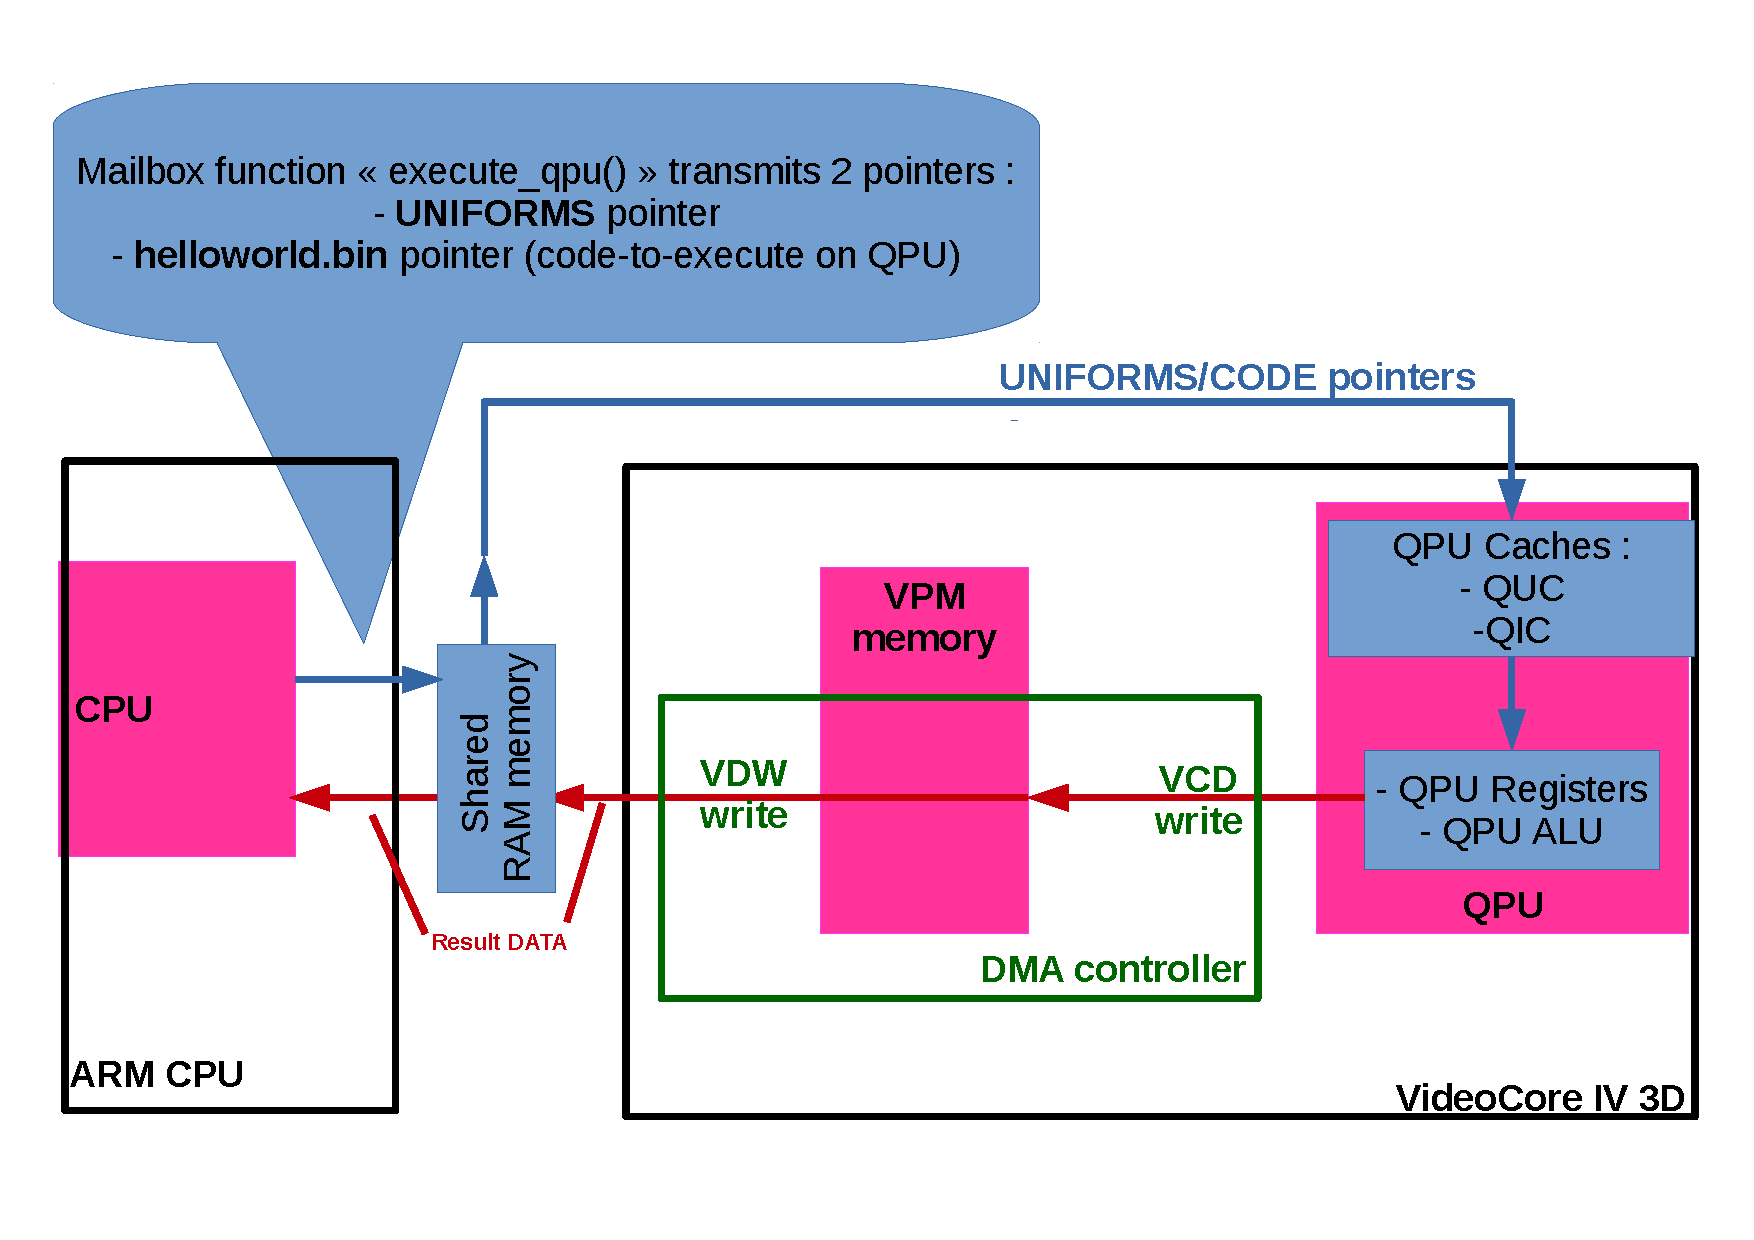
\includegraphics[width=0.9\textwidth]{helloworldDataFlow}
	\caption{\file{helloworld} execution diagram}
	\label{flowFigure}
\end{figure}
\FloatBarrier


Figure~\ref{flowFigure} sums up the \file{helloworld} program execution:

\begin{itemize}
	\item We use two \uni{}s to transfer an \emph{input value} (100) and a pointer to \emph{results array address} - \code{results[NUM\_QPUS][16]} - from the host \cpu{} to the \emph{QPU 0,0}
	\item We send them with \code{execute\_qpu()}, a \mail{} function.
	\item These 2 uniforms will be load into \emph{QUC : Uniforms Cache}.
	\item We also tranfer a pointer to the \code{code-to-execute} on \keyword{GPU}.
	\item \code{code-to-execute} is then load into \emph{QIC : Icache (Instructions cache)}.
	\item \emph{QPU 0,0} adds \emph{100} to \emph{0x1234}.
	\item First, the result (16-word vector) is write back to \keyword{VPM}.
	\item Then, the result (16-word vector) is write back from \keyword{VPM} to \ram{} memory through \keyword{DMA} transfer.
\end{itemize}


\subsection{Conclusion}\label{GPUconclusion}

This project taught me the basis of \vc{} programming and laid the groundwork for the rest of my internship. I understood that:
\begin{itemize}
	\item GPU and CPU share the same RAM memory - Appendice~\ref{AppendixB}
		\begin{itemize}
			\item CPU sends code \keyword{pointers} and variables called \uni{}s in the \emph{VC CPU Bus Addresses}
			\item GPU gives back results in \emph{VC CPU Bus Addresses}
			\item CPU gets results since \emph{ARM Virtual Addresses} and \emph{VC CPU Bus Addresses} are bind together with \code{mapmem()}
		\end{itemize}
	\item GPU is driven by CPU program (\file{driver.c}) that:
		\begin{itemize}
			\item initialize GPU
			\item map \ram{} memory and bind \emph{ARM Virtual Addresses} \& \emph{VC CPU Bus Addresses}
			\item copy code and data in the \ram
			\item send code pointers and variables called \uni{}s in the \emph{VC CPU Bus Addresses}
			\item get back results
		\end{itemize}
	\item GPU and CPU communicate via \mail{}:
		\begin{itemize}
			\item \api{} that uses low-level linux kernel functions
			\item source code is available in the raspbian distribution
		\end{itemize}
	\item GPU processor is called \qpu{} -- Appendice~\ref{AppendixD}:
		\begin{itemize}
			\item SIMD processors -- operates on 16-words vector
			\item 12 QPUs on \vc
		\end{itemize}
	\item GPU is fitted with - Appendice~\ref{AppendixC}:
		\begin{itemize}
			\item VPM to store result from QPU
			\item DMA to send result from VPM to \ram{} memory
		\end{itemize}
	\item To run program on GPU:
		\begin{itemize}
			\item \code{code-to-execute} is written in \keyword{assembly language} - \file{helloworld.asm}
			\item \code{code-to-execute} is translate into \keyword{binary} file - \file{helloworld.bin}
			\item \code{code-to-execute} is copied in \ram{} by the \cpu
			\item \code{code-to-execute} pointer is sent to \keyword{GPU}
			\item \code{variables} called \uni{}s are sent to \qpu{}
			\item \vc{} gives back in the \emph{VC CPU Bus Addresses}
		\end{itemize}
\end{itemize}
To build the homemade \api{} for \iBubble, I focused on:
\begin{itemize}
	\item improve \file{driver.c}
	\item refactore project architecture
	\item use a more comprehensive \code{assembly parser} than \file{assemble.cpp}
	\item find new \vc{} features
	\item include my source code in \keyword{C++} project
\end{itemize}

%----------------------------------------------------------------------------------------

\section{Standard Project}

\subsection{\emph{pi-gemm} Project}

\emph{pi-gemm} \parencite{refPiGemm} is a project written by Pete \textsc{Warden} with associated \file{github}: \url{https://github.com/jetpacapp/pi-gemm}. It implements optimized \emph{GEMM} algorithm on \vc.

This project is interesting for several reasons:
\begin{itemize}
	\item the author wrote an improved \code{assembly parser} -- \file{qpu-asm.cpp}
	\item \emph{pi-gemm} introduces the \keyword{TMU} -- Appendice~\ref{AppendixC}
	\item multiply matrix is massively used in \flow{} processing
	\item \emph{pi-gemm} algorithm is called in a \file{main.cpp} file -- as our homemade \api
	\item \emph{pi-gemm} \file{Makefile} is more generic
\end{itemize}


\subsection{Texture Memory Unit and Matrices}\label{Matrices}

\emph{pi-gemm} introduces the way to use matrices and \keyword{TMU}, a new crucial component of \vc{}.

\keyword{TMU} enables \qpu{} to directly access data from the \ram{}. We just have to pass data pointer from the \emph{VC CPU Bus Addresses} in some \keyword{uniforms} variables to load the values containing at this address.

For instance, matrices which are stored in the \ram{} can be accessed knowing the pointer of the first element. I also noticed that matrices are stored in \emph{row-major} order (Figure~\ref{rowcolumnarrays}). That means row values are contiguous in \ram{} memory. This is a \keyword{key point} to know because frames from the \rasp{} camera are stored as \option{float-matrices} in memory and to compute the \flow{} we have to access data from those frames.

\begin{figure}[!htbp]
	\centering
	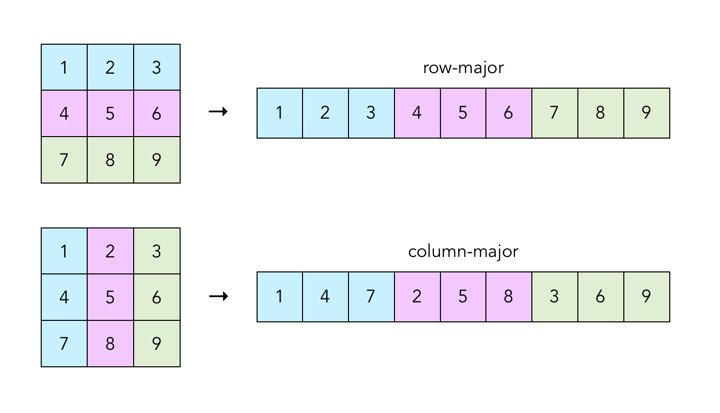
\includegraphics[width=0.6\textwidth]{rowcolumnarrays}
	\caption{Row-major vs. Colon-major matrices}
	\label{rowcolumnarrays}
\end{figure}
\FloatBarrier


\subsection{Refactoring projects}

My goal while studying \emph{pi-gemm} project was to create a standard framework to develop my own projects. I finally came with a mix between both \file{helloworld} and \file{pi-gemm} projects. Figure~\ref{projectArchitectureFigure} shows my project architecture:

\begin{figure}[!htbp]
	\centering
	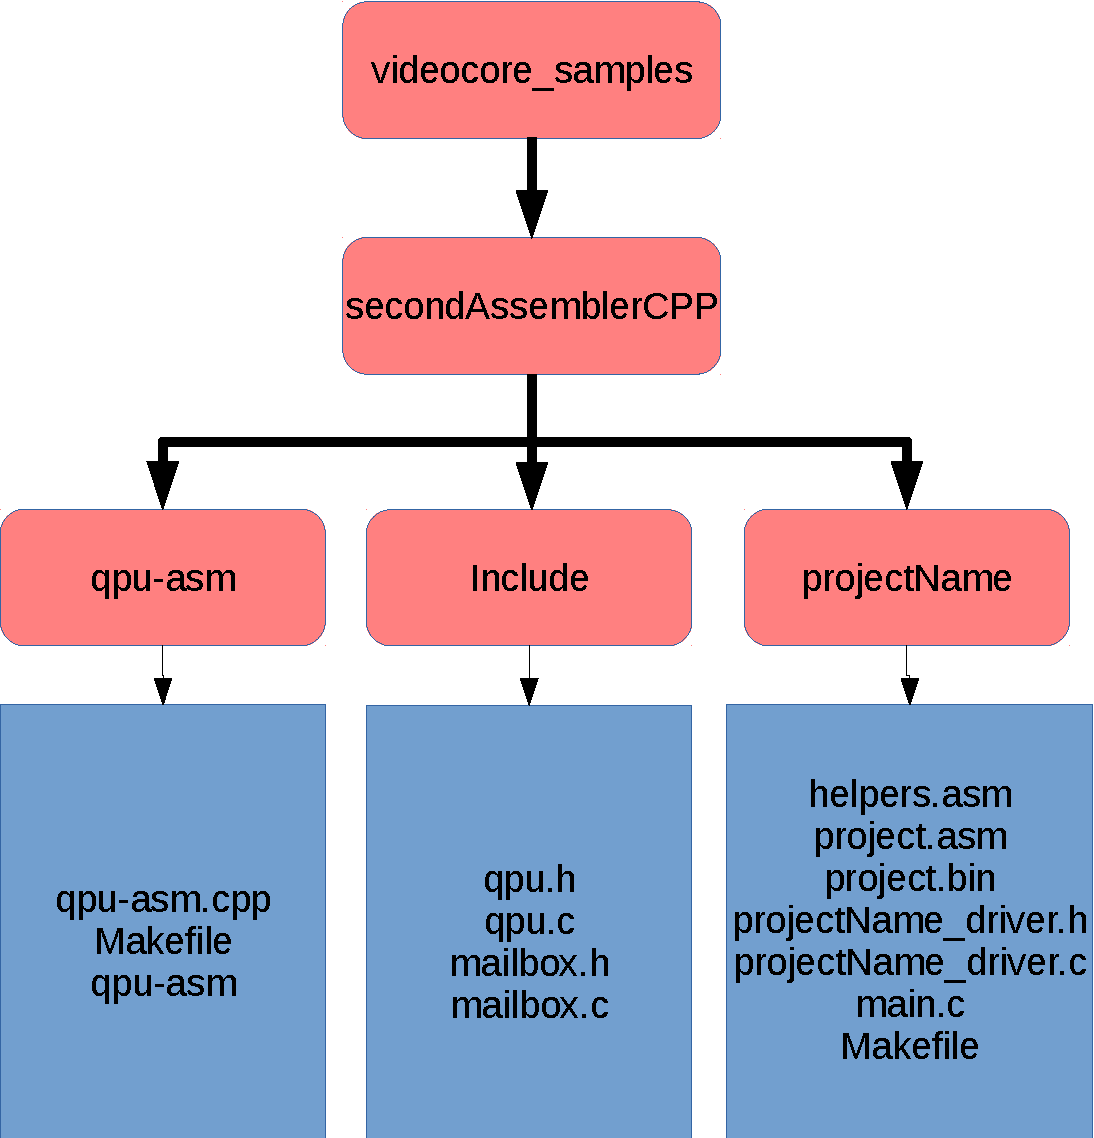
\includegraphics[width=0.4\textwidth,scale=0.2]{projectArchitecture}
	\caption{Standard Framework Project Architecture}
	\label{projectArchitectureFigure}
\end{figure}
\FloatBarrier


\subsubsection{qpu-asm}

This directory contains 3 files: \file{qpu-asm.cpp}, \file{Makefile}, and \file{qpu-asm}.

\file{qpu-asm.cpp} is the \code{assembly parser} from \file{pi-gemm} written by Pete \textsc{Warden}. It is more comprhensive because it features more instructions of the \vc.

\lstset{language=make,caption={},captionpos=t,label=}
\begin{lstlisting}
qpu-assembler: assemble.cpp
	g++ -g -o qpu-assembler assemble.cpp
\end{lstlisting}

Run the \code{make} command will generate \file{qpu-asm}, an \keyword{executable} file and then:\\
\begin{center}
\code{./qpu-asm -o projectName.bin < projectName.asm}
\end{center}


\subsubsection{Include}

This directory contains 4 files: \file{qpu.h}, \file{qpu.c}, \file{mailbox.h} and \file{mailbox.c}.
Those files are included into the \emph{Raspbian Stretch Lite} distribution and allow us to use the \mail{} interface to communicate between \vc{} and \cpu.

I included \mail{} source code directly in this directory for more software portabilty.

\subsubsection{projectName}

\file{projectName} directory contains:
\begin{itemize}
	\item \file{project.asm}/\file{project.bin} -- \code{code-to-execute} on \vc.
	\item \file{projectName\_driver.h}/\file{projectName\_driver.c} -- \keyword{GPU} driver that contains functions to map memory, send data and code to \vc{} etc \ldots
	\item \file{main.c} -- invoke functions from \file{projectName\_driver.c} to run \code{code-to-execute} on \vc.
	\item \file{Makefile} -- generic \file{Makefile} that generates an \keyword{executable} called \file{projectName} - Appendice~\ref{AppendixF}.
\end{itemize}


\subsubsection{Run project}
\lstset{language=make,caption={},captionpos=t,label=}
\begin{lstlisting}
cd qpu-asm
make qpu-asm
cd projectName
make
sudo ./projectName
\end{lstlisting}


\subsubsection{Project Examples}

Once this standard framework was running well, I started developping several projects to run on the \rasp. The goal was to learn more \vc{}'s features and architecture. For instance I developped programs that:
\begin{itemize}
	\item take two 16-word vectors from \cpu{} memory, copy and multiply them inside \ram{} and give back result to \cpu
	\item take a $(240\times 360)float-matrix$ from \cpu{} memory, copy it inside \ram{}, convoluate it by a $(3\times 3)kernel$ and give back the resulting $(238\times 358)float-matrix$ to \cpu
\end{itemize}
\newpage

%----------------------------------------------------------------------------------------

\section{Other Abilities}\label{FillingFile}

In addition to my research on \vc{}'s projects, I developped several other helpful skills in software development during this internship.


\subsection{Linux \& Vim}

At \groupname{} the software developpment is done using GNU/Linux OS. Thus I used \emph{GCC} or \emph{G++} compilers and I got immersed in Linux Architecture, Command Line or in Makefile writting. I also needed to compile some libraries (\emph{Python, OpenCV} from scratch and face some compiling error after hours of running.

Since I developped on \rasp{}, I started using \emph{Vim} editor. Nicolas \textsc{Vincent} a member of the embedded software team, conviced me to start using this very \emph{customizable} editor. He learned me the basis and how to add useful plug-ins. He was a great adviser for me and taught me a lot of tricks.


\subsection{git \& github}

Another very helpful skill I gained during my internship is in \emph{git} and \emph{github} using. I started to use \code{git clone} to copy projects on my \rasp.

Within \groupname{} I created my first professional \emph{repository} called \keyword{videocore\_samples}: \url{https://github.com/notiloPlus/videocore_samples}. In this repository I put all the projects I developped to explore the \vc.

I made this repository very teaching in order to learn other people how to use \vc. To do that, I wrote my \emph{README.md} file to explain how to use this repository. I had to learn how to write \file{markdown(.md)} files.

I maintained this repository using \code{git add}, \code{git commit} and \code{git push} commands.


\subsection{\LaTeX}

When came time to write this report I decided to use \LaTeX{}. I found a template that I customized to fill my needs. I didn't use any IDE but I added a \LaTeX{} plug-in to \emph{Vim} to continue learning how to use this editor. It was my first major report written in \LaTeX{} so the beginning was harsh. Nevertheless, I finished without any compiling errors and the result is very stylish.

%----------------------------------------------------------------------------------------

\section{Conclusion}\label{Conclusion2}

At the end of this internship work, I was more confortable to deal with my internship subject. So I started developping the \api{} to use \vc. I had more interactions with Camille to build the \flow{} project. 

% Chapter 4

\chapter{Internship Subject} % Main chapter title

\label{Chapter3} % For referencing the chapter elsewhere, use \ref{Chapter3}

%----------------------------------------------------------------------------------------

% Define some commands to keep the formatting separated from the content
%\newcommand{\keyword}[1]{\textbf{#1}}
%\newcommand{\tabhead}[1]{\textbf{#1}}
%\newcommand{\code}[1]{\texttt{#1}}
%\newcommand{\file}[1]{\texttt{\bfseries#1}}
%\newcommand{\option}[1]{\texttt{\itshape#1}}

%----------------------------------------------------------------------------------------

\section{Problematics}

As I said in the previous parts, \iBubble{} includes a visual tracking system, \keyword{CMT}, to \emph{autonomously} follow divers underwater. This system currently uses \emph{openCV} libraries at a rate of \textbf{30 fps}. This speed can be improved using \emph{CUDA} technology. These feat{}s are only available on \keyword{BtB} versions of \iBubble{} fitted with \emph{Nvidia's Jetson embedded board}.

\keyword{BtC} versions of the drone uses \rasp{} in spite of the current \emph{Nvidia Graphics Card} wich means that \emph{CUDA} is no longer available because \vc{} is not designed with this technology.

As a consequence, \vc{} is not used so the whole tracking system is running only on the \cpu{} and the system rate drops to \textbf{7 fps}.

The more time-consuming part of the \keyword{CMT} is the \flow{} computation. This is a fundamental tracking algorithm in Computer Vision. It uses \keyword{Gradient Descent} and \keyword{Pyramid} algorithms to get the displacement of the points of interest between two frames.

Therefore if we want to use the computing power of the \vc{}, it is compulsory to make our own implementation of the \flow{} on \rasp, that was my internship subject.

The main difficulty is that there is no official \keyword{API} released by \textsc{Broadcom}. To compute the \flow{} on \rasp, it was to necessary to follow the same steps as in Chapter~\ref{Chapter2}, namely:
\begin{itemize}
	\item write \code{code-to-execute} on \keyword{GPU} -- in \option{assembly language}
	\item parse this \code{code-to-execute} with \keyword{assembly parser} -- \file{qpu-asm.cpp}
	\item write a \code{driver program} for the \keyword{CPU} -- in \option{c-language}
	\item include this \keyword{API} in a \option{C++} project -- \keyword{CMT} is written in \option{C++}
\end{itemize}

%----------------------------------------------------------------------------------------

\section{Optical Flow}

\subsection{Definition}

Within \iBubble{} visual tracking system - \keyword{CMT} - \flow{} is the displacement of points of interest - called \feat{}s - between two consecutive frames from a video.

Computing \emph{optical flow} between two consecutive frames involves the following steps:
\begin{itemize}
	\item detect \feat{}s on first image -- Figure~\ref{initFeaturesFig}
	\item find the next \feat{}s positions on the second image -- Figure~\ref{secondFeaturesFig}
	\item compute \emph{displacemnt} for each \feat{}s -- Figure~\ref{opticalFlowFig}
\end{itemize}


\begin{figure}[!htbp]
	\centering
	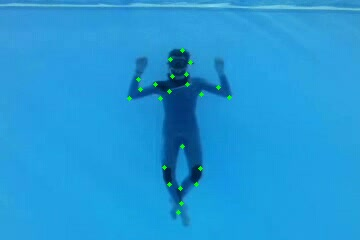
\includegraphics[width=0.5\textwidth]{plongeurInitFeatures}
	\caption{First frame of a diving video with the initial set of \feat{}s}
	\label{initFeaturesFig}
\end{figure}
\FloatBarrier



\begin{figure}[!htbp]
	\centering
	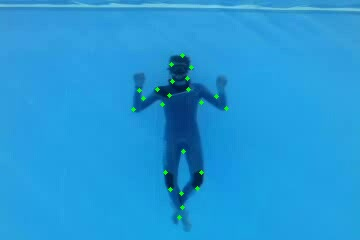
\includegraphics[width=0.5\textwidth]{plongeurNextFeatures}
	\caption{Second frame of a diving video with new \feat{}s positions}
	\label{secondFeaturesFig}
\end{figure}
\FloatBarrier



\begin{figure}[!htbp]
	\centering
	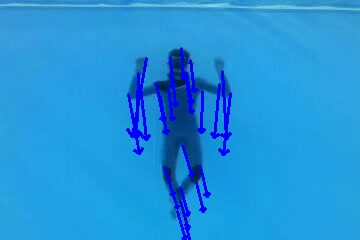
\includegraphics[width=0.5\textwidth]{plongeurOpticalFlow}
	\caption{Optical flow for the initial set of \feat{}s -- \small{norm of the \textcolor{blue}{blue vectors} is overstated for better visualization}}
	\label{opticalFlowFig}
\end{figure}
\FloatBarrier

\emph{Optical flow} can be viewed as a \emph{vector field} representing \feat{}s displacement between two consecutive frames. It is used to do object recognition, tracking or movement detection. In \iBubble, \emph{optical flow} is compute within \keyword{CMT} to achieve diver \emph{autonomous tracking and following}.\par


\subsection{Images encoding}

As I mentioned in~\ref{Matrices}, frames from the \rasp's camera (Figures~\ref{initFeaturesFig} to ~\ref{opticalFlowFig}) are \option{row major float-matrices}. More specifically, a frame is a ($240\times 360$) pixel array:

\begin{figure}[!htbp]
\[
\begin{bmatrix}

pixel_{0,0} & pixel_{0,1} & \ldots & \ldots & \ldots & pixel_{0,359}\\

pixel_{1,0} & \ddots & \ldots & \ldots & \ldots & pixel_{1,359}\\

\vdots & \ldots & \ddots & \ldots & \ldots & \vdots\\

\vdots & \ldots & \ldots & \cellcolor{yellow}{feature_{x,y}} & \ldots & \vdots\\

\vdots & \ldots & \ldots & \ldots & \ddots & \vdots\\

pixel_{239,0} & \ldots & \ldots  & \ldots & \ldots & pixel_{239,359}

\end{bmatrix}_{240\times 360}
\]
\caption{Frame from camera: two-dimensionnal pixel array}
\label{frameFig}
\end{figure}
\FloatBarrier

Moreover, \flow{} algorithm uses \emph{grayscale} images:

\begin{itemize}
	\item each $pixel_{x,y}$ is encoded as \option{32-bit float}
	\item stored at @$pixel_{x,y}$ address
	\item @$pixel_{x,y}$ is a \option{32-bit integer} -- Appendice~\ref{AppendixB}
\end{itemize}


From the shared RAM point of view, a frame is a contiguous array:
\begin{figure}[h]
\begin{center}
\begin{tabular}{|c|c|c|}

	\hline
	\begin{bf}$\text{@pixel}_\text{{x,y}}$\end{bf} & \begin{bf}offset\end{bf} & \begin{bf}$\text{@pixel}_\text{{x,y}}$\end{bf} \\[10pt]

	\hline
	@$pixel_{0,0}$ & @$pixel_{0,0}$ & $pixel_{0,0}$ \\

	\hline
	@$pixel_{0,1}$ & @$pixel_{0,0} + 4$ & $pixel_{0,1}$ \\

	\hline
	\vdots & \vdots & \vdots \\

	\hline
	@$pixel_{0,359}$ & @$pixel_{0,0} + 359\times 4$ & $pixel_{0,359}$ \\

	\hline
	@$pixel_{1,0}$ & @$pixel_{0,0} + 1\times 360$ & $pixel_{1,0}$ \\

	\hline
	@$pixel_{1,1}$ & @$pixel_{0,0} + 1\times 360 + 1\times 4$ & $pixel_{1,1}$ \\

	\hline
	\vdots & \vdots & \vdots \\

	\hline
	\rowcolor{yellow}@$pixel_{x,y}$ & @$pixel_{0,0} + x\times 360 + y\times 4$ & $pixel_{x,y}$ \\

	\hline
	\vdots & \vdots & \vdots \\

	\hline
	@$pixel_{x,y}$ & @$pixel_{0,0} + 239\times 360 + 359\times 4$ & $pixel_{239,359}$ \\

	\hline

\end{tabular}
\end{center}
\caption{Contiguous Array in Memory}
\end{figure}
\FloatBarrier

As a result to access particular $pixel_{x,y}$ value with the \qpu, we must pass 3 parameters to the \vc's \keyword{TMU}:
\begin{itemize}
	\item @$pixel_{0,0}$ -- starting address of the frame in the \emph{VC CPU Bus Addresses}
	\item $x$ -- pixel row number
	\item $y$ -- pixel coloumn number
\end{itemize}

Within a frame, a \feat{} is a specific $pixel$ with specific $(x,y)$ numbers (Figure~\ref{frameFig}). To know the \option{32-bit float value} of $feature_{x,y}$, we must pass those 3 parameters to the \keyword{TMU}.


\subsection{Parameters, Notations and Expected Outcomes}


\subsubsection{Parameters}

Before invoking the \flow{} computation, the \emph{tracking system} must provide three parameters to the \vc:

\begin{itemize}
	\item first frame data -- must be a pointer to the first pixel $\textcolor{blue}{firstFrame_{0,0}}$
	\item 30 $feature_{x,y}$ positions -- must be a pointer to an integer array: \file{int} $featuresArray[2][30]$
	\item second frame data -- must be a pointer to the first pixel $\textcolor{red}{secondFrame_{0,0}}$
\end{itemize}


\subsubsection{Notations}

All notations are summarized on Figure~\ref{framesWindowFig}.

A pixel from first frame will be noted $\textcolor{blue}{firstFrame_{x,y}}$.\\
A pixel from second frame will be noted $\textcolor{red}{secondFrame_{x,y}}$.\\
A pixel from window in firstFrame will be noted $\textcolor{blue}{firstWindow_{x,y}}$.\\
A pixel from window in secondFrame will be noted $\textcolor{red}{secondWindow_{x,y}}$.\\
A feature \keyword{row number} will be noted $\textcolor{blue}{x_{1}}$ on \textcolor{blue}{firstFrame} and $\textcolor{red}{x_{2}}$ on \textcolor{red}{secondFrame}.\\
A feature \keyword{column number} will be noted $\textcolor{blue}{x_{1}}$ on \textcolor{blue}{firstFrame} and $\textcolor{red}{x_{2}}$ on \textcolor{red}{secondFrame}.\\
Finally, the \keyword{same feature} will be noted $feature_{\textcolor{blue}{y_{1},y_{1}}}$ on \textcolor{blue}{firstFrame} and $feature_{\textcolor{red}{x_{1},y_{1}}}$ on \textcolor{red}{secondFrame}.

\subsubsection{Expected Outcomes}

The expected results of the \flow{} algorithm are written Figure~\ref{framesWindowFig}. For each \feat{}, the \vc{} must compute:
\begin{itemize}
	\item \textbf{$d_{x}$} -- the feature displacement along the row axis measured in pixel: $\textcolor{red}{x_{2}}-\textcolor{blue}{x_{1}}$
	\item \textbf{$d_{y}$} -- the feature displacement along the column axis measured in pixel: $\textcolor{red}{y_{2}}-\textcolor{blue}{y_{1}}$
\end{itemize}

So the \flow{} program will return a \file{float} $displacementsArray[2][30]$ containing:
\begin{itemize}
	\item 30 $d_{x}$ \option{float values} -- one for each feature
	\item 30 $d_{y}$ \option{float values} -- one for each feature
\end{itemize}

This is the \flow{} between two consecutive frames for 30 \feat{}s.


\subsubsection{Summary}

To summarize the \flow{} computation between two consecutive frames for each feature on \vc:
\begin{itemize}
	\item inputs:
		\begin{itemize}
			\item $\textcolor{blue}{firstFrame_{0,0}}$ pointer
			\item $\textcolor{red}{secondFrame_{0,0}}$ pointer
			\item \file{int} $featuresArray[2][30]$
		\end{itemize}
	\item outputs: \file{float} $displacementsArray[2][30]$
\end{itemize}

\begin{figure}[!htbp]
	\centering
	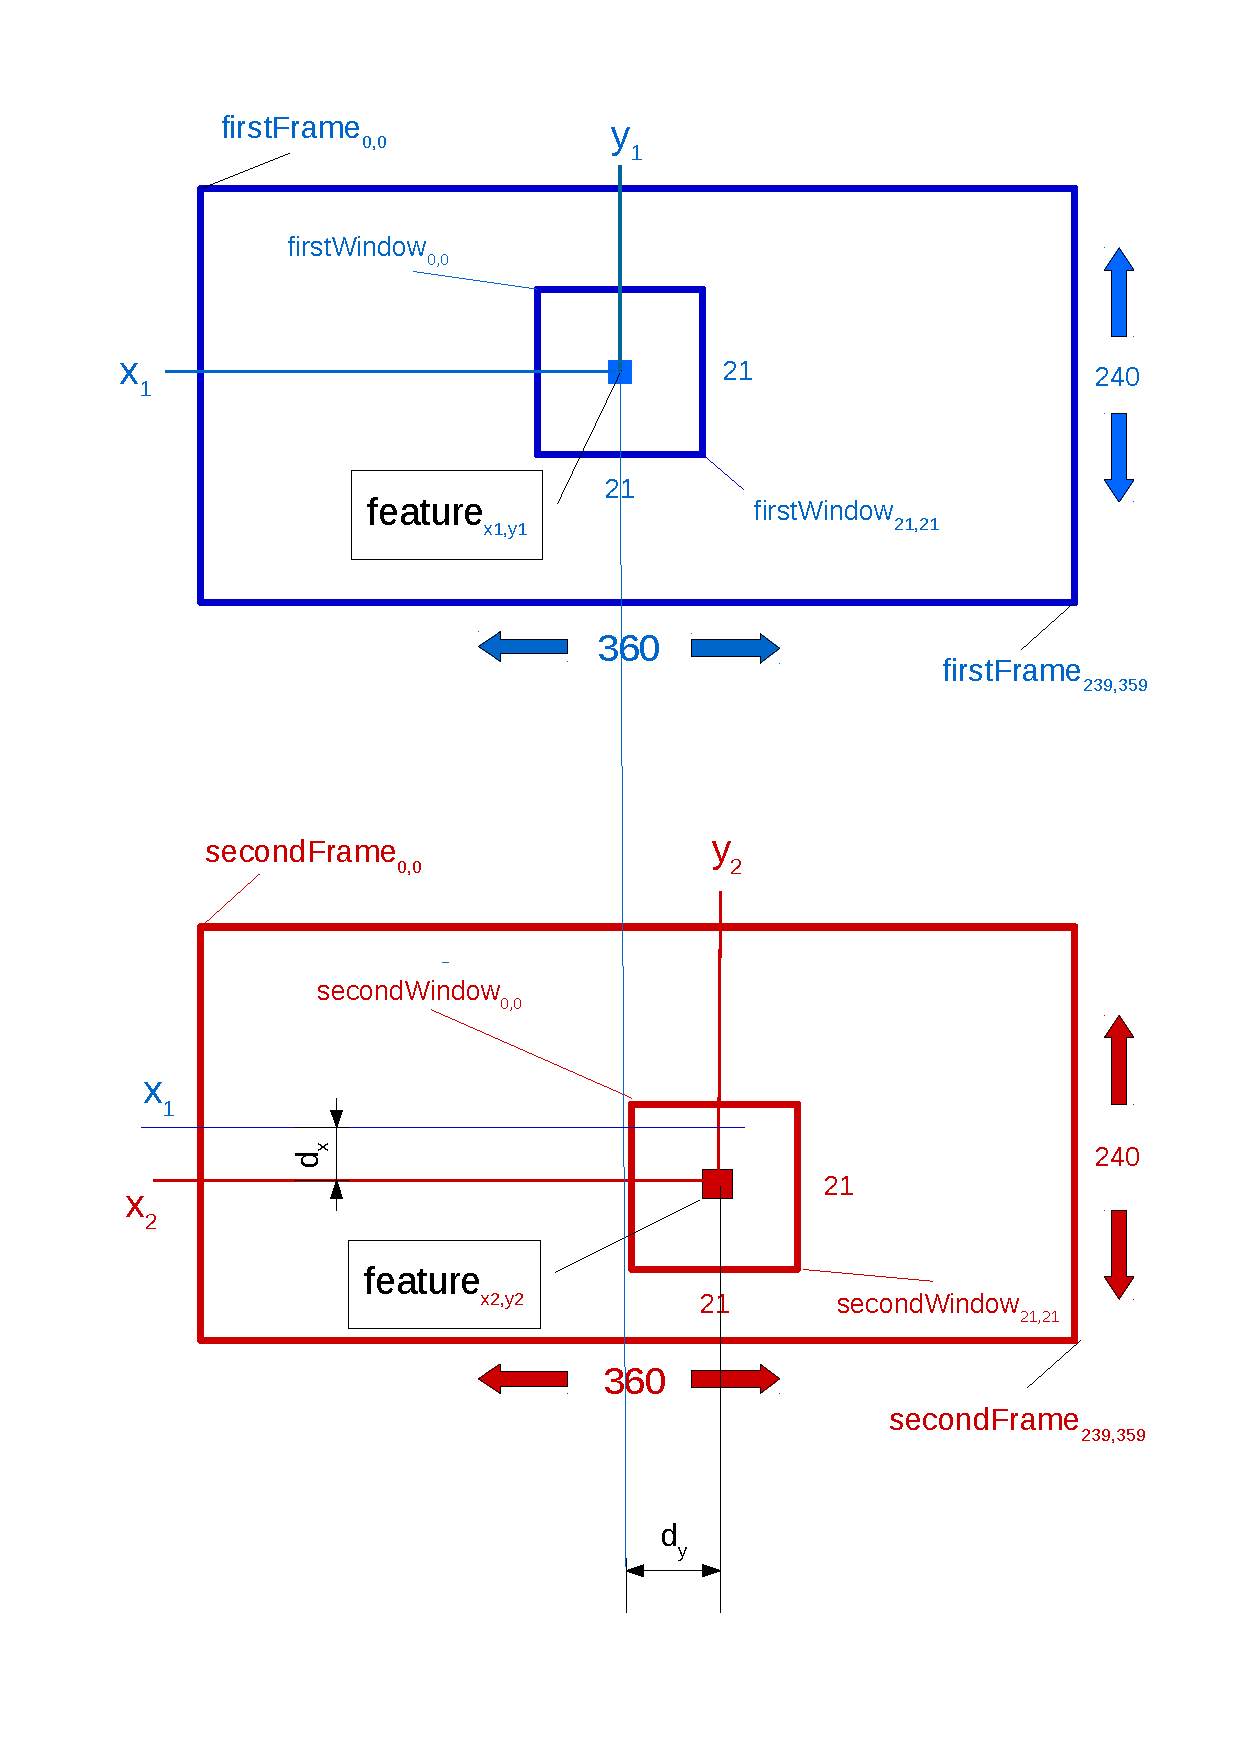
\includegraphics[width=0.8\textwidth]{framesWindow}
	\caption{Optical flow between \textcolor{blue}{first frame} and \textcolor{red}{second frame} for one feature}
	\label{framesWindowFig}
\end{figure}
\FloatBarrier

%----------------------------------------------------------------------------------------

\section{Lucas-Kanade method}

There are several ways to compute \flow{}. Camille selected \keyword{Lucas-Kanade} method to be implemented on \vc.

The \emph{vision tracking} algorithm detects \keyword{30} feat{}s on each frame from the camera. Thus, our \emph{homemade} algorithm must compute \flow{} for these 30 feat{}s between two consecutive frames.

Although there are 30 feat{}s, I will present the Lucas-Kanade method for one \feat{}, $feature_{x,y}$. The processing is the same for the rest of the feat{}s.

For the rest of this section, keep in mind Figure~\ref{framesWindowFig}.

\subsection{First Frame Processing}

When \vc{} gets $\textcolor{blue}{firstFrame_{0,0}}$, \file{int} $featuresArray[2][30]$ and $\textcolor{red}{secondFrame_{0,0}}$ he starts processing the first frame.

The goal is to get 4 values per \feat{}:
\begin{itemize}
	\item $G_{XX}$ -- vertical gradient of the feature
	\item $G_{YY}$ -- horizontal gradient of the feature
	\item $G_{XY}$ -- cross gradient of the feature
	\item $det = \frac{1}{G_{XX}G_{YY}-G_{XY}G_{XX}}$
\end{itemize}

As shown in Figure~\ref{framesWindowFig}, we use a $21\times21$ \option{pixel window} around the feature:

$$G_{XX} = \sum_{i=1}^{21}\sum_{j=1}^{21} grad_{x}[i,j]^{2}$$
$$G_{YY} = \sum_{i=1}^{21}\sum_{j=1}^{21} grad_{y}[i,j]^{2}$$
$$G_{XY} = \sum_{i=1}^{21}\sum_{j=1}^{21} grad_{x}[i,j]\times grad_{y}[i,j]$$

Where, for a pixel element - $firstWindow_{i,j}$ -  of the window:
$$grad_{x}[i,j] = \frac{firstWindow_{i+1,j} - firstWindow_{i-1,j}}{2}$$
$$grad_{y}[i,j] = \frac{firstWindow_{i,j+1} - firstWindow_{i,j-1}}{2}$$


\subsection{Displacement computation}

To compute the feature displacement, we use the following algorithm:

\begin{figure}[!htbp]
\begin{algorithmic}
	\ForAll {$firstWindow_{i,j}$ and $secondWindow_{i,j}$}

	\State $diff\_frames = firstWindow_{i,j} - secondWindow_{i+d_{x},j+d_{y}}$

	\State $frames\_mismatch.x = diff\_frames\times grad_{x}[i,j]$
	\State $frames\_mismatch.y = diff\_frames\times grad_{y}[i,j]$

	\EndFor

	\State $d_{x} = det\times (G_{YY}\times frames\_mismatch.x - G_{XY}\times frames\_mismatch.y)$
	\State $d_{y} = det\times (G_{XX}\times frames\_mismatch.y - G_{XY}\times frames\_mismatch.x)$
\end{algorithmic}
\caption{Displacement algorithm for one feature}
\label{algoFig}
\end{figure}
\FloatBarrier

The algorithm Figure~\ref{algoFig} is running several times to have a better precision on $d_{x}$ and $d_{y}$ values. Each time, we reinject previous $d_{x}$ and $d_{y}$ to compute $\textcolor{red}{secondWindow_{i+d_{x},j+d_{y}}}$. Results analysis shows that for a little feature displacement, 5 times is enough to have better precision than \emph{OpenCV} function.\\


Within the displacement algorithm, $\textcolor{red}{secondWindow_{i+d_{x},j+d_{y}}}$ is a \emph{bilinear interpolation}:

\begin{figure}[!htbp]
\begin{equation*}
	\begin{split}
		secondWindow_{i+d_{x},j+d_{y}} = secondWindow_{floor(i+d_{x}),floor(j+d_{y})}\times (1-fract(i+d_{x}))\times (1-fract(i+d_{y}))\\
		+ secondWindow_{floor(i+d_{x})+1,floor(j+d_{y})}\times (fract(i+d_{x}))\times (1-fract(i+d_{y}))\\
		+ secondWindow_{floor(i+d_{x}),floor(j+d_{y})+1}\times (1-fract(i+d_{x}))\times (fract(i+d_{y}))\\
		+ secondWindow_{floor(i+d_{x})+1,floor(j+d_{y})+1} \times (fract(i+d_{x}))\times (fract(i+d_{x}))
	\end{split}
\end{equation*}
\caption{Bilinear interpolation within second frame window}
\label{BIPFig}
\end{figure}
\FloatBarrier

The \emph{bilinear interpolation} Figure~\ref{BIPFig} was though to achieve with the \vc{} because it needs \option{floor} and \option{fractional functions} that are not native in this \keyword{GPU}. To do so I used \code{ftoi}, \code{itof}, and \code{fsub} functions Figure~\ref{VCinstructionsFigure}.


Camille detailed me those algorithm on a big white board (Appendice~\ref{AppendixA}) and implemented them in \keyword{C++}. Then it was easier for me to translate them into \option{assembly language}.

%----------------------------------------------------------------------------------------

\section{Current Solution \& testing framework}

\subsection{Current Solution}

The \flow{} computation is used within the \keyword{CMT} algorithm for \iBubble's \emph{visual tracking system}. Currently, the tracking system invokes an \emph{OpenCV} function: \code{calcOpticalFlowPyrLK()}.

The main objective of Camille and I's internships was to write an homemade \code{calcOpticalFlowPyrLK()} function that invokes the \vc{} to parallelize some computing tasks and so, free resources of \cpu. In our homemade \keyword{API} the name of this function is \code{compute\_lk\_gpu()}.


\subsection{Testing framework}

Camille provided me a comprehensive testing environment to test my \keyword{API}. It was a whole \keyword{C++} project using \keyword{CMake} program. The project name was \file{optical\_flow\_internship} and I just had to \code{clone} this project from the \file{gitHub} platform. To run the project I followed the standard \code{CMake} procedure:


\lstset{language=make,caption={CMake for optical\_flow\_internship framework},label=}

\begin{lstlisting}
cd optical_flow_internship
mkdir build && cd build
cmake..
make
sudo ./optical_flow_internship /path_to_video_sample
\end{lstlisting}

\code{cmake ..} followed by \code{make} generates \file{optical\_flow\_internship}, an \keyword{executable} file that takes a path to a \emph{video\_sample}. The program computes the \flow{} between each consecutive frames of the sample until the end of the video. The sample was an underwater video from \iBubble. Figures~\ref{initFeaturesFig} to ~\ref{opticalFlowFig} are fames from this sample.

In this framework, 3 \file{files} concerne my \api{}:
\begin{itemize}
	\item \file{opt\_flow\_lk.cpp} -- where I write \code{compute\_lk\_gpu()}.
	\item \file{opt\_flow\_video.cpp} -- where \code{compute\_lk\_gpu()} is invoked.
	\item \file{main.cpp} -- the \code{main} program that process the \emph{video\_sample}.
\end{itemize}

\lstset{style=CStyle,caption={Select between OpenCV and \vc},label=selectList}

\begin{lstlisting}
if (this->use_opencv_lk_)
{
	calcOpticalFlowPyrLK(prev_gray, gray, points[0], points[1], status,
        this->max_iterations_, cpt);
}
else if (this->use_lk_gpu_)
{
	this->estim_flow.compute_lk_gpu(prev_gray, gray, points[0], points[1], status,
	this->max_iterations_, cpt);
}
\end{lstlisting}

Listing~\ref{selectList} taken from \file{opt\_flow\_video.cpp} shows how we can choose between \code{calcOpticalFlowPyrLK()} and \code{compute\_lk\_gpu()} to compute \flow.

Both functions takes the same input parameters:
\begin{itemize}
	\item \keyword{prev\_gray} -- firstFrame
	\item \keyword{gray} -- secondFrame
	\item \keyword{points[0]} -- array containing 30 initial \feat{}s (x,y) positions
	\item \keyword{points[1]} -- array containing 30 (dx, dy) displacements
	\item \keyword{status} -- parameter needed for the rest of the tracking
	\item \keyword{max\_iterations} -- number of times that displacement algorithm is invoked
	\item \keyword{cpt} -- number of frame in the \emph{video\_sample}
\end{itemize}
%----------------------------------------------------------------------------------------

\section{Implementation on \vc}

\subsection{Architecture}

\subsection{invoke GPU function}
I followed the same method as in the previous part~\ref{GPUconclusion} invoke GPU.

My driver (grad.c) will:
\begin{itemize}
	\item initialize \qpu{}s
	\item map the \ram
	\item copy code and data (frames 1 and 2 and featuresArray) in \ram
	\item send code pointer and \uni{}s
	\item get back the results
\end{itemize}


%% Conclusion

\chapter{Conclusion} % Main chapter title

\label{Conclusion} % For referencing the chapter elsewhere, use \ref{Conclusion}

%----------------------------------------------------------------------------------------

% Define some commands to keep the formatting separated from the content
%\newcommand{\keyword}[1]{\textbf{#1}}
%\newcommand{\tabhead}[1]{\textbf{#1}}
%\newcommand{\code}[1]{\texttt{#1}}
%\newcommand{\code}[1]{\texttt{\hl{#1}}}
%\newcommand{\file}[1]{\texttt{\bfseries#1}}
%\newcommand{\option}[1]{\texttt{\itshape#1}}
%\newcommand{\iBubble}{\textsc{iBubble}}
%\newcommand{\rasp}{\textsc{Raspberry Pi}}
%\newcommand{\vc}{\textsc{VideoCore iv 3D}}
%\newcommand{\cpu}{\textsc{arm cpu}}
%\newcommand{\bcm}{\textsc{bcm2837}}
%\newcommand{\qpu}{\textsc{qpu}}
%\newcommand{\flow}{\textsc{optical flow}}
%\newcommand{\feat}{\textsc{feature}}
%\newcommand{\api}{\textsc{api}}
%\newcommand{\ram}{\textsc{shared ram}}
%\newcommand{\mail}{\textsc{mailbox}}
%\newcommand{\uni}{\textsc{uniform}}

%----------------------------------------------------------------------------------------

\section{Results}

To test this \api{} I compute the \flow{} first using \code{calcOpticalFlowPyrLK()} and then using \code{compute\_lk\_gpu()}: listing~\ref{mainLst}. Running the project with \code{sudo ./optical\_flow\_internship /home/pi/video/video\_out.avi} generates a directory containing three files:
\begin{itemize}
	\item \file{video\_out\_init\_features.jpg}: an image containing the initial \feat{}s positions - Figure~\ref{initFeaturesFig}
	\item \file{video\_out\_opt\_flow\_vectors.avi}: a video where \flow{} between each consecutive frames is representing by \textcolor{blue}{blue vectors} - Figure~\ref{opticalFlowFig}
	\item \file{video\_out\_vectors.json}: a \file{.json} file containing all the 30 $(d_{x},d_{y})$ values for each frame of the whole \emph{video\_sample}
\end{itemize}

Moreover the terminal displays time processing for each frame of the video. So I am able to compare time when using this two functions.


\subsection{Time Comparison}

\lstset{language=bash,caption={\code{calcOpticalFlowPyrLK} terminal output},basicstyle=\tiny,label=}
\begin{lstlisting}
mean time per frame: 0.00538982 for 24 frames.
JSON file of vectors of each features at each frames can be found at: /home/pi/video/video_out/video_out_vectors.json

Video with vector representing optical flow has been written at : /home/pi/video/video_out/video_out_opt_flow_vectors.avi

**********************************************************************
**********************************************************************
All videos / frames of: /home/pi/video have been processed !
**********************************************************************
\end{lstlisting}


\lstset{language=bash,caption={\code{calcOpticalFlowPyrLK} terminal output},basicstyle=\tiny,label=}
\begin{lstlisting}
mean time per frame: 0.0119438 for 24 frames.
JSON file of vectors of each features at each frames can be found at: /home/pi/video/video_out/video_out_vectors.json

Video with vector representing optical flow has been written at : /home/pi/video/video_out/video_out_opt_flow_vectors.avi

**********************************************************************
**********************************************************************
All videos / frames of: /home/pi/video have been processed !
**********************************************************************
\end{lstlisting}



\subsection{Values Comparison}

\noindent\begin{minipage}{.45\textwidth}
\begin{lstlisting}[caption={\code{calcOpticalFlowPyrLK} values},frame=tlrb,basicstyle=\tiny]{Name}
"number": "9",
"vectors": {
	"feature 1": "[0.00437927, 1.01498]",
	"feature 2": "[0.0429688, 0.984863]",
	"feature 3": "[-0.00196838, 0.985191]",
	"feature 4": "[0.013916, 0.999466]",
	"feature 5": "[-0.00466919, 1.02369]",
	"feature 6": "[0.00923157, 1.59529]",
	"feature 7": "[0.136581, 1.39946]",
	"feature 8": "[0.320084, 1.5918]",
	"feature 9": "[0.0149536, 1.03059]",
	"feature 10": "[-0.0966644, 1.72192]",
	"feature 11": "[0.00205994, 0.997665]",
	"feature 12": "[0.175995, 1.14218]",
	"feature 13": "[-0.0109406, 1.09407]",
	"feature 14": "[0.0992737, 1.05608]",
	"feature 15": "[0.205734, 1.56096]",
	"feature 16": "[0.0429688, 1.02802]",
	"feature 17": "[0.243973, 1.51352]",
	"feature 18": "[0.0153656, 1.83011]",
	"feature 19": "[0.0600433, 1.05858]",
	"feature 20": "[-0.000396729, 1.00053]",
	"feature 21": "[0.0501404, 1.38897]",
	"feature 22": "[0.12709, 1.79247]",
	"feature 23": "[0.289734, 2.45174]",
	"feature 24": "[0.0285187, 0.95536]",
	"feature 25": "[0.161499, 1.30433]",
	"feature 26": "[0.12973, 1.23988]",
	"feature 27": "[0.108826, 0.860413]",
	"feature 28": "[0, 0]",
	"feature 29": "[0, 0]",
	"feature 30": "[0, 0]"
}
\end{lstlisting}
\end{minipage}\hfill
\begin{minipage}{.45\textwidth}
	\begin{lstlisting}[caption={\code{compute\_lk\_gpu} values},frame=tlrb,basicstyle=\tiny]{Name}
"number": "9",
"vectors": {
	"feature 1": "[0.0307007, 1.05986]",
	"feature 2": "[0.0518036, 1.08145]",
	"feature 3": "[0.00424194, 1.06021]",
	"feature 4": "[0.015625, 1.01106]",
	"feature 5": "[0.00361633, 0.998215]",
	"feature 6": "[-0.0257874, 1.5815]",
	"feature 7": "[0.249847, 1.38773]",
	"feature 8": "[0.265816, 1.47562]",
	"feature 9": "[0.00706482, 0.996964]",
	"feature 10": "[-0.0304565, 1.66684]",
	"feature 11": "[0.0141449, 0.985558]",
	"feature 12": "[0.0645599, 1.18579]",
	"feature 13": "[0.0774689, 1.00171]",
	"feature 14": "[0.0397186, 1.09403]",
	"feature 15": "[-0.0235443, 1.05531]",
	"feature 16": "[0.0857086, 1.01047]",
	"feature 17": "[0.14328, 1.62175]",
	"feature 18": "[-0.0360718, 1.74749]",
	"feature 19": "[0.0405731, 1.0332]",
	"feature 20": "[-0.0058136, 0.991623]",
	"feature 21": "[0.0559845, 1.42413]",
	"feature 22": "[0.00138855, 1.08983]",
	"feature 23": "[0.00791931, 0.980244]",
	"feature 24": "[-0.0236969, 1.04613]",
	"feature 25": "[-0.0176392, 1.65675]",
	"feature 26": "[0.0956726, 1.2908]",
	"feature 27": "[0.0596008, 1.01413]",
	"feature 28": "[0.00686646, 0.994537]",
	"feature 29": "[-0.0133667, 1.12775]",
	"feature 30": "[-0.00701904, 2.02641]"
}
\end{lstlisting}
\end{minipage}


%----------------------------------------------------------------------------------------

\section{Possibilities}

As of the writing of this report, a part of the Lucas-Kanade method was still in development. This part called \emph{Gaussian Pyramids} is a way to estimate large displacement - large values of $(d_{x},d_{y})$ - between two frames.

Inputs are still \textcolor{blue}{firstFrame}, \textcolor{red}{secondFrame} and \file{int} $featuresArray[2][30]$. The \emph{Gaussian Pyramids} algorithm is invoked before displacement computation section~\ref{dispComp}. This algorithm provides initial approached values of the $(d_{x},d_{y})$ for each feature. Those values are injected on the first iteration of displacement computation.

\subsection{Pyramid Algorithm}

\subsubsection{First convolution}

\noindent\begin{minipage}{.3\textwidth}
\[
\begin{bmatrix}

firstPixel_{0,0} & firstPixel_{0,1} & \ldots & \ldots & firstPixel_{0,359}\\

firstPixel_{1,0} & \ddots & \ldots & \ldots & firstPixel_{1,359}\\

\vdots & \ldots & \ddots & \ldots & \vdots\\

\vdots & \ldots & \ldots & \ddots & \vdots\\

firstPixel_{239,0} & \ldots & \ldots  & \ldots & firstPixel_{239,359}

\end{bmatrix}_{240\times 360}
\]
\end{minipage}\hfill
\begin{minipage}{.3\textwidth}
\[
\begin{bmatrix}

1 & 2 & 1\\

2 & 4 & 2\\

1 & 2 & 1\\

\end{bmatrix}_{3\times 3 kernel}
\]
\end{minipage}


\subsubsection{Second convolution}

\noindent\begin{minipage}{.3\textwidth}
\[
\begin{bmatrix}

secondPixel_{0,0} & secondPixel_{0,1} & \ldots & \ldots & secondPixel_{0,357}\\

secondPixel_{1,0} & \ddots & \ldots & \ldots & secondPixel_{1,357}\\

\vdots & \ldots & \ddots & \ldots & \vdots\\

\vdots & \ldots & \ldots & \ddots & \vdots\\

secondPixel_{237,0} & \ldots & \ldots  & \ldots & secondPixel_{237,357}

\end{bmatrix}_{238\times 358}
\]
\end{minipage}\hfill
\begin{minipage}{.3\textwidth}
\[
\begin{bmatrix}

1 & 2 & 1\\

2 & 4 & 2\\

1 & 2 & 1\\

\end{bmatrix}_{3\times 3 kernel}
\]
\end{minipage}


\subsubsection{Extraction}

\[
\begin{bmatrix}

thirdPixel_{0,0} & thirdPixel_{0,1} & \ldots & \ldots & thirdPixel_{0,355}\\

thirdPixel_{1,0} & \ddots & \ldots & \ldots & thirdPixel_{1,355}\\

\vdots & \ldots & \ddots & \ldots & \vdots\\

\vdots & \ldots & \ldots & \ddots & \vdots\\

thirdPixel_{235,0} & \ldots & \ldots  & \ldots & thirdPixel_{117,355}

\end{bmatrix}_{236\times 356}
\]



\[
\begin{bmatrix}

thirdPixel_{0,0} & thirdPixel_{0,2} & \ldots & \ldots & thirdPixel_{0,354}\\

thirdPixel_{2,0} & \ddots & \ldots & \ldots & thirdPixel_{2,354}\\

\vdots & \ldots & \ddots & \ldots & \vdots\\

\vdots & \ldots & \ldots & \ddots & \vdots\\

thirdPixel_{234,0} & \ldots & \ldots  & \ldots & thirdPixel_{234,354}

\end{bmatrix}_{118\times 178}
\]

\subsubsection{Optical flow algorithm}

Once we get the $118\times 178$ matrix from first and second frame, we apply the \flow{} the same way as in ~\ref{Chapter3} with all values of features posions divided by two.

We get 30 $d_{x},d_{y}$ approached values of the features displacement and we can start the \flow{} algorithm for the $240\times 360$ first and second frame to get the exact values of the displacement.
%----------------------------------------------------------------------------------------


%\include{Chapters/Chapter5}

%----------------------------------------------------------------------------------------
%	THESIS CONTENT - APPENDICES
%----------------------------------------------------------------------------------------

\appendix % Cue to tell LaTeX that the following "chapters" are Appendices

% Include the appendices of the thesis as separate files from the Appendices folder
% Uncomment the lines as you write the Appendices

% Appendix A

\chapter{Optical Flow} % Main appendix title

\label{AppendixA} % For referencing this appendix elsewhere, use \ref{AppendixA}

\section{First frame gradient}

\begin{figure}[!htbp]
\centering
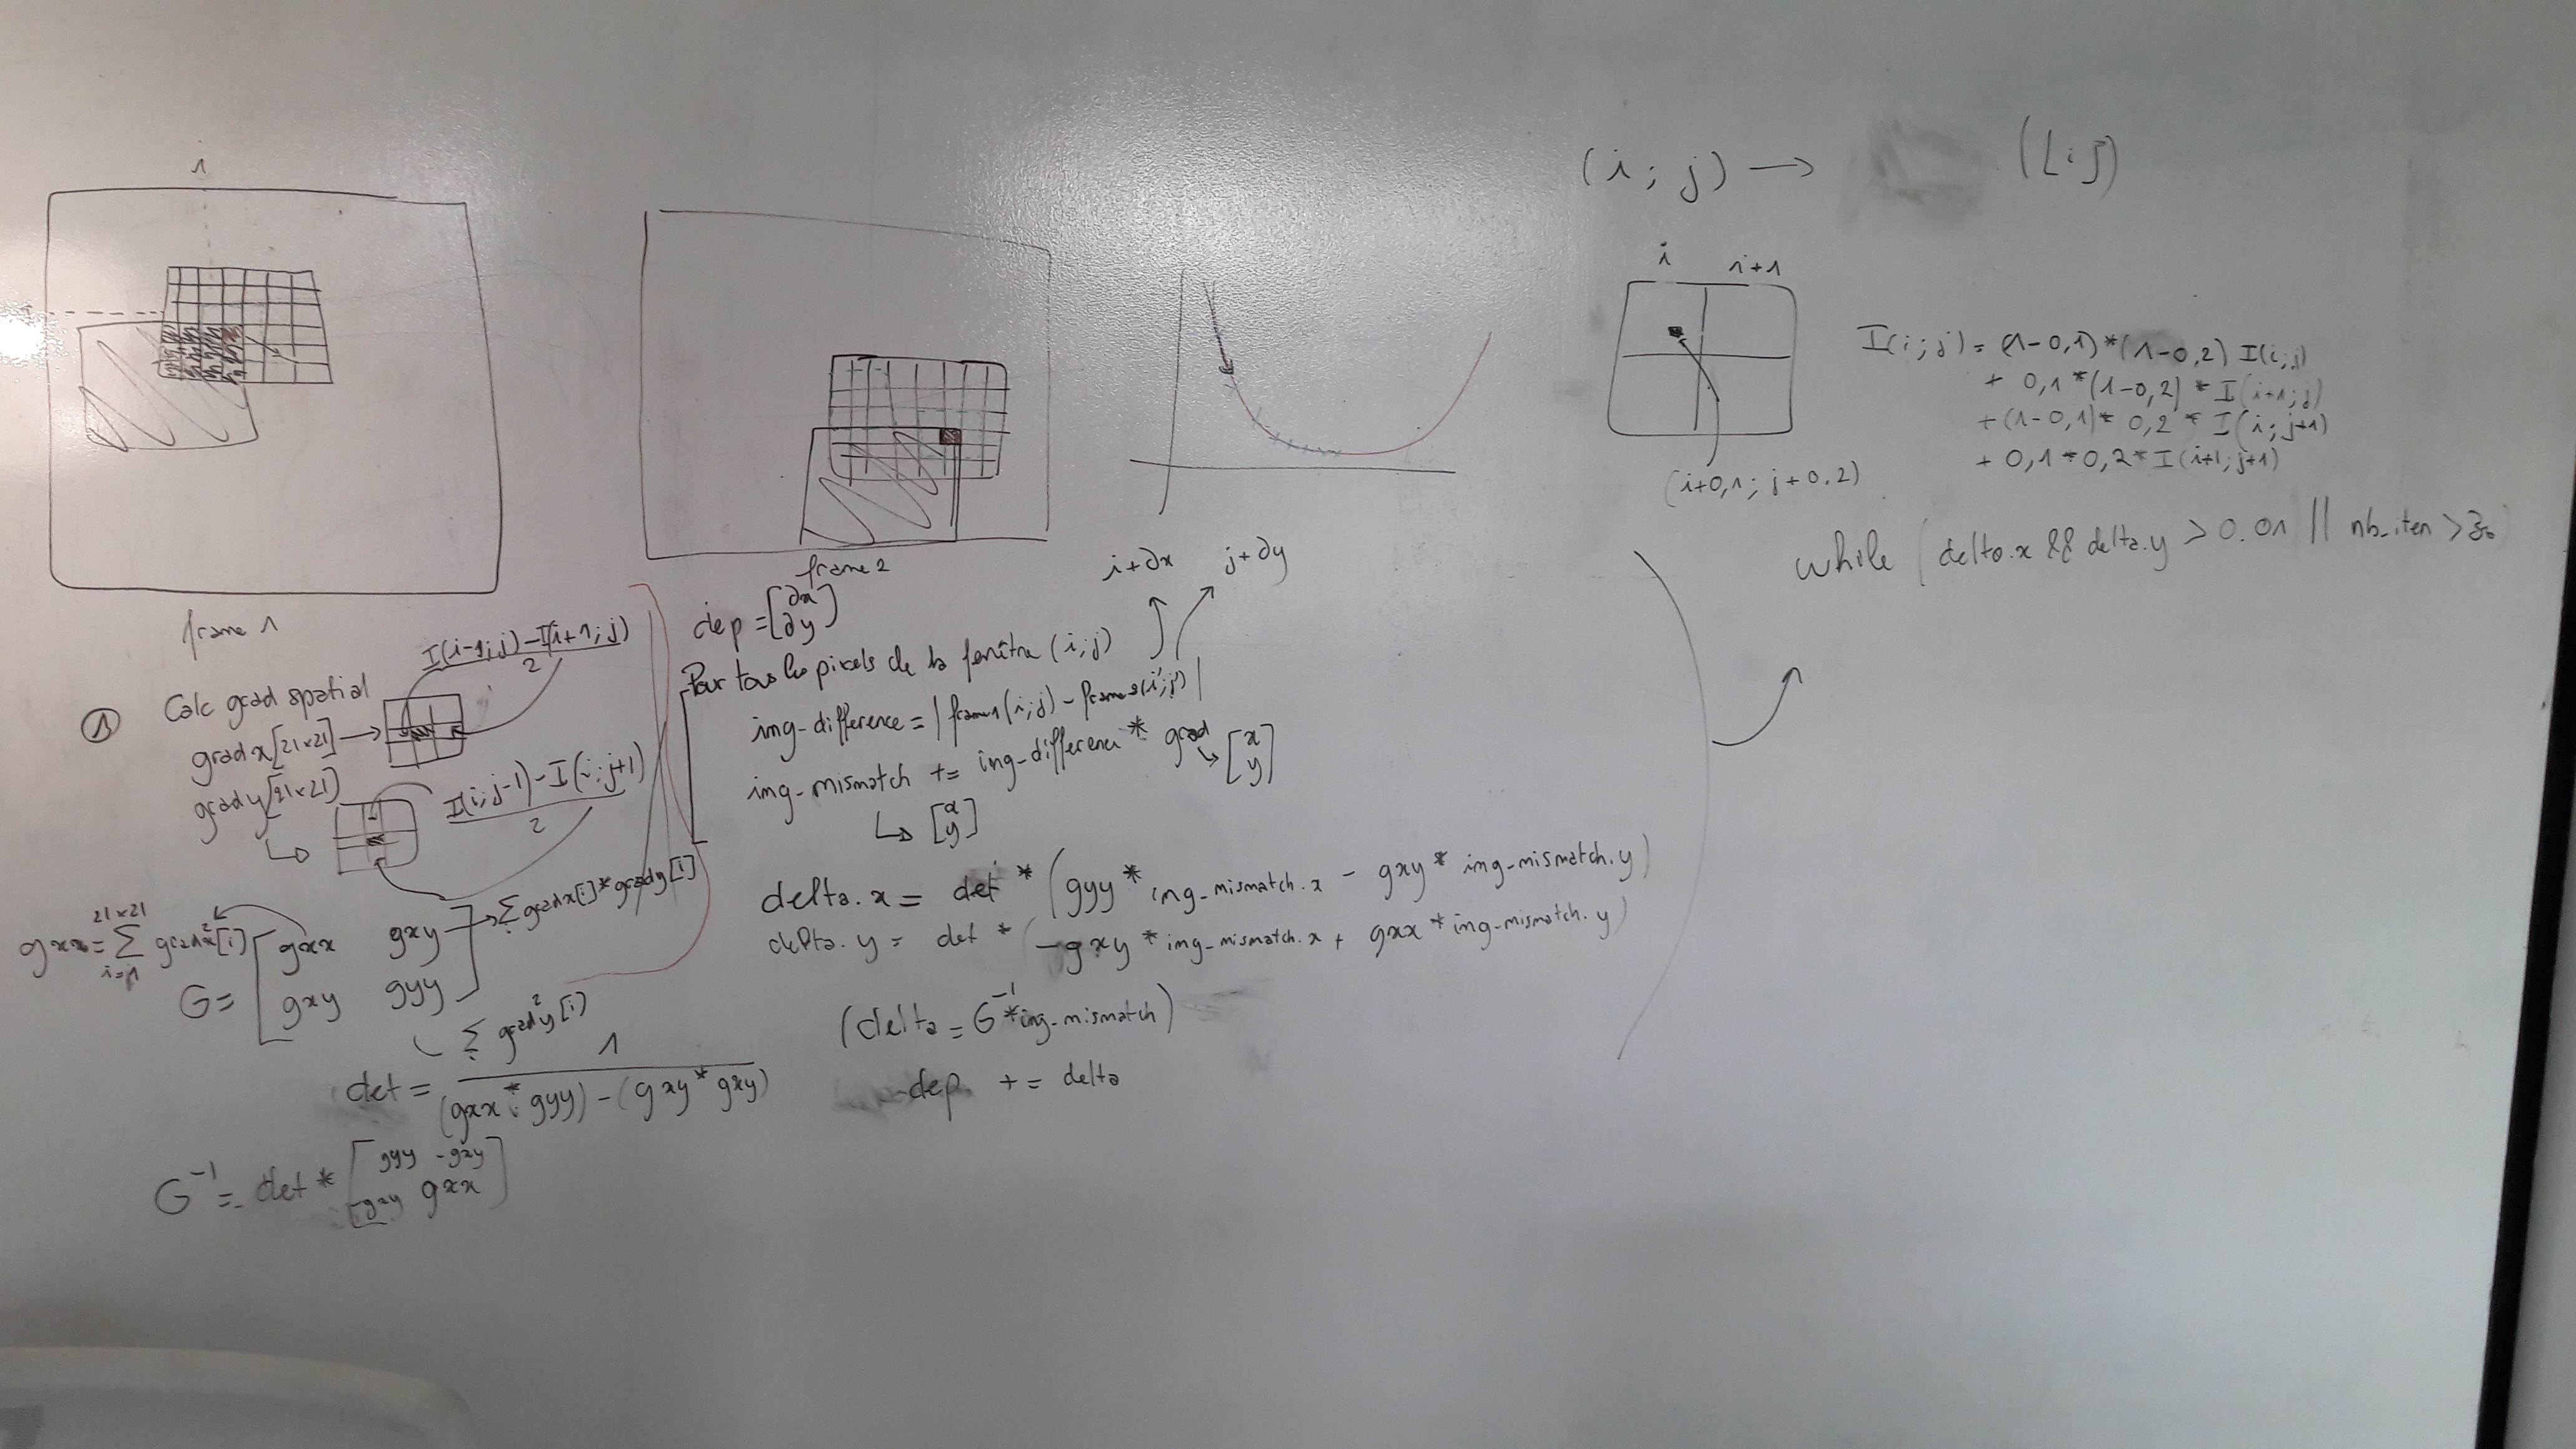
\includegraphics[width=0.9\textwidth]{gradFirstFrame1}
%\caption{\vc{} and \cpu{} Shared RAM}
%\label{sharedFigure}
\end{figure}


\section{Displacement algorithm}

\begin{figure}[!htbp]
\centering
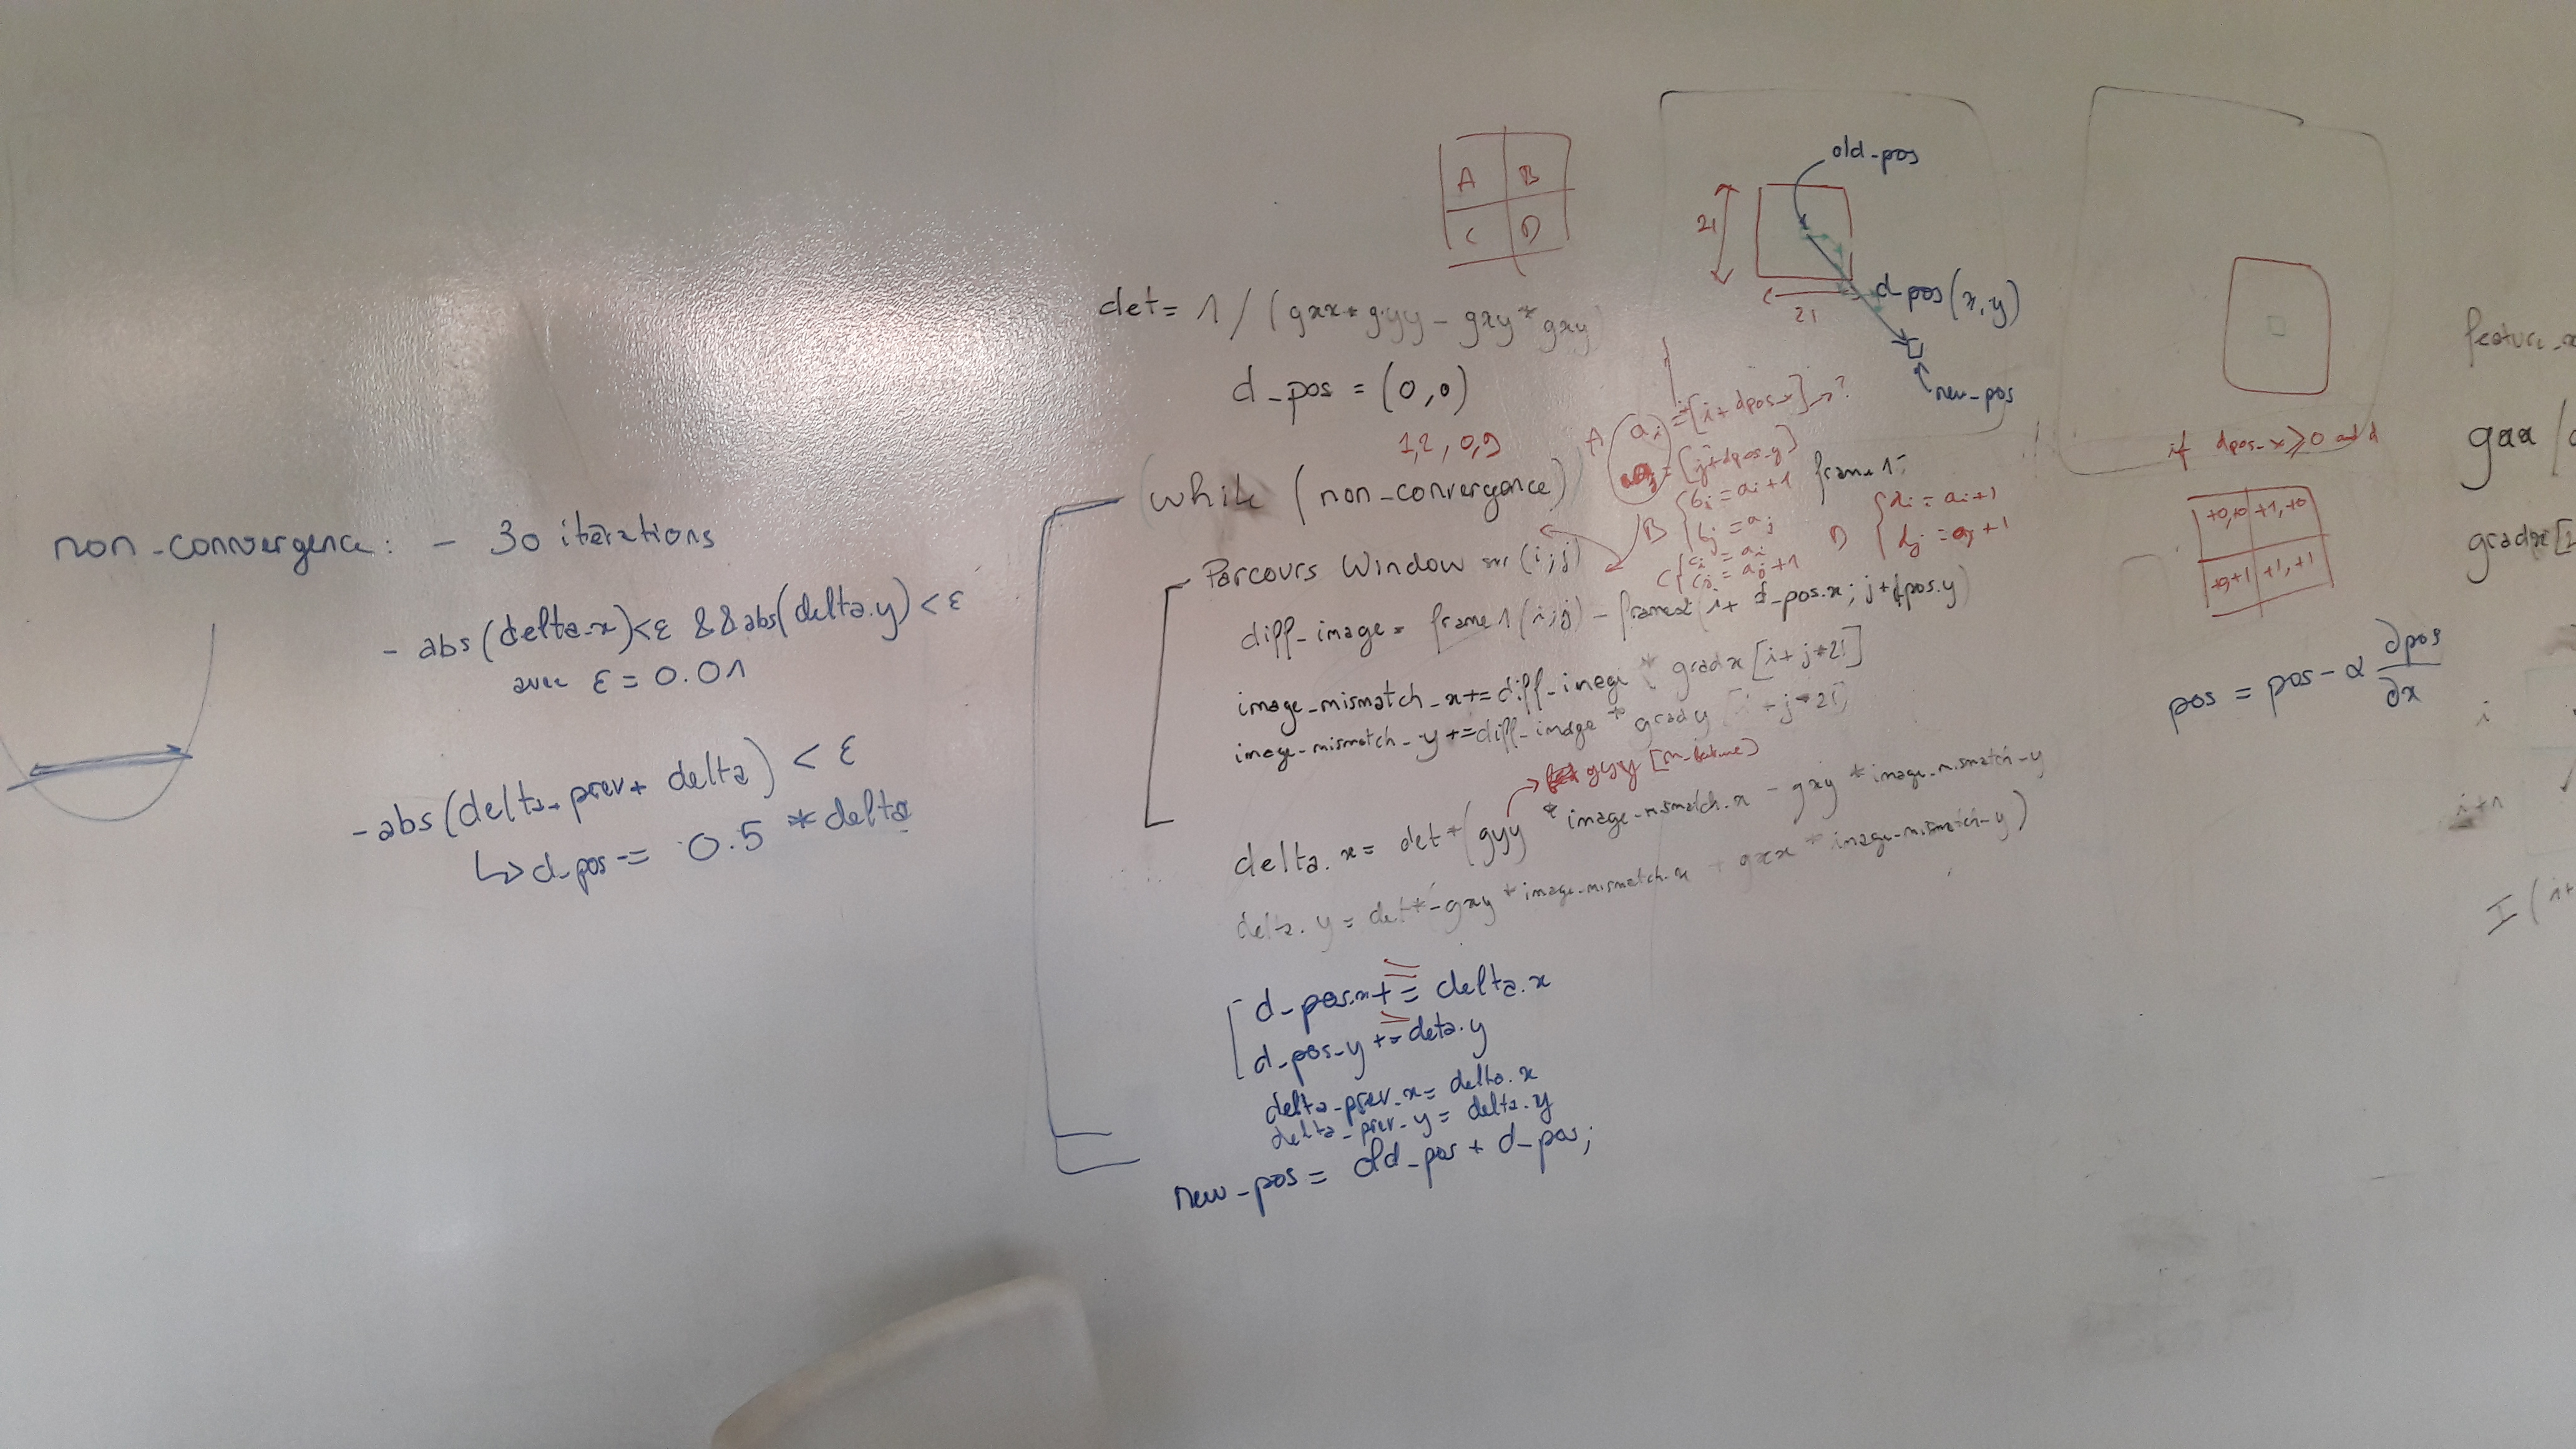
\includegraphics[width=0.9\textwidth]{displacementLoop1}
%\caption{\vc{} and \cpu{} Shared RAM}
%\label{sharedFigure}
\end{figure}

% Appendix B

\chapter{\bcm{} \ram{} memory} % Main appendix title

\label{AppendixB} % For referencing this appendix elsewhere, use \ref{AppendixB}

\begin{figure}[!htbp]
\centering
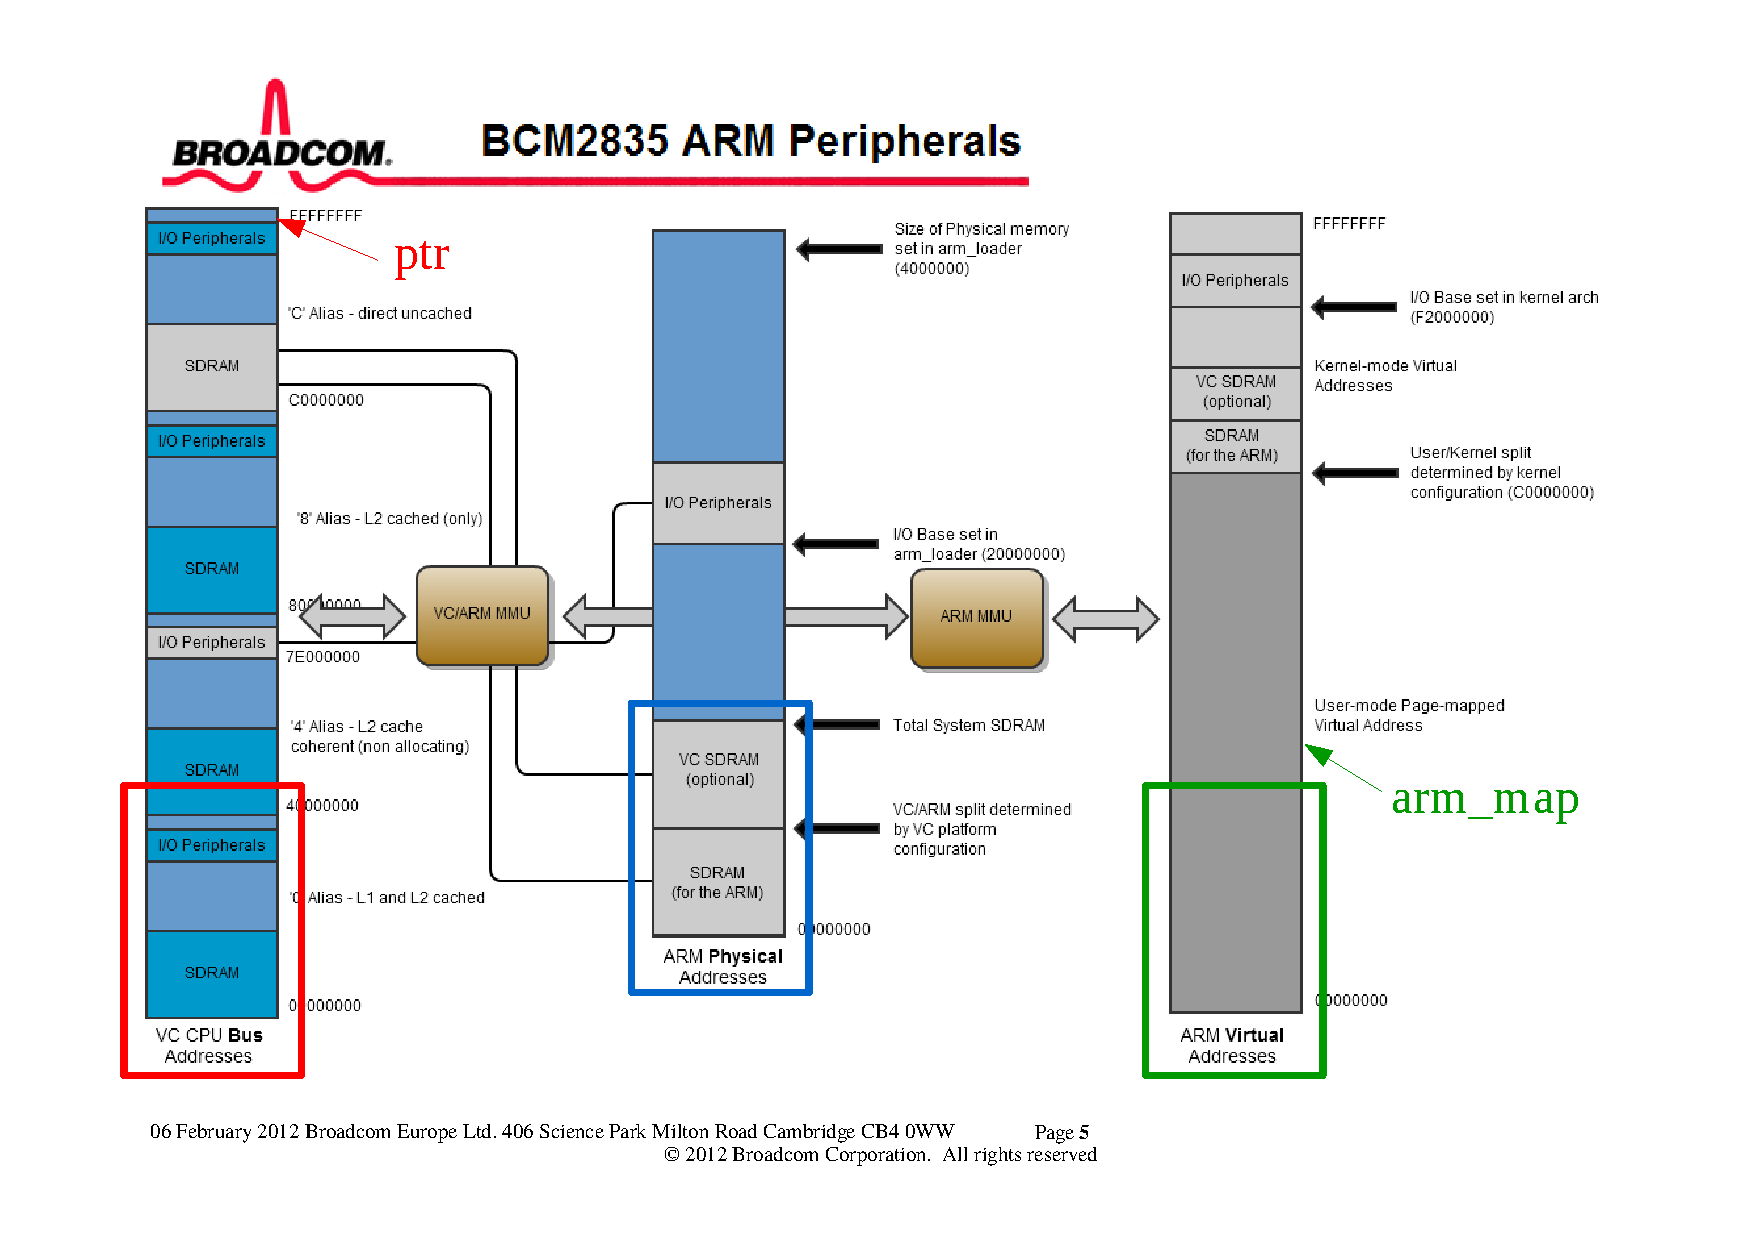
\includegraphics[width=\textwidth]{RAMptrs}
%\caption{\vc{} and \cpu{} Shared RAM}
%\label{sharedFigure}
\end{figure}

\textsc{Notes}:

-- The underlying architecture of the \bcm{} is identical to the BCM2835. The only significant difference is the replacement of the ARMv7 quad core cluster with a quad-core ARM Cortex A53 (ARMv8) cluster.\\

-- \bcm{} and BCM2835 are both fitted with \vc.


% Appendix C

\chapter{\vc{} Overview} % Main appendix title

\label{AppendixC} % For referencing this appendix elsewhere, use \ref{AppendixB}

\begin{figure}[!htbp]
	\centering
	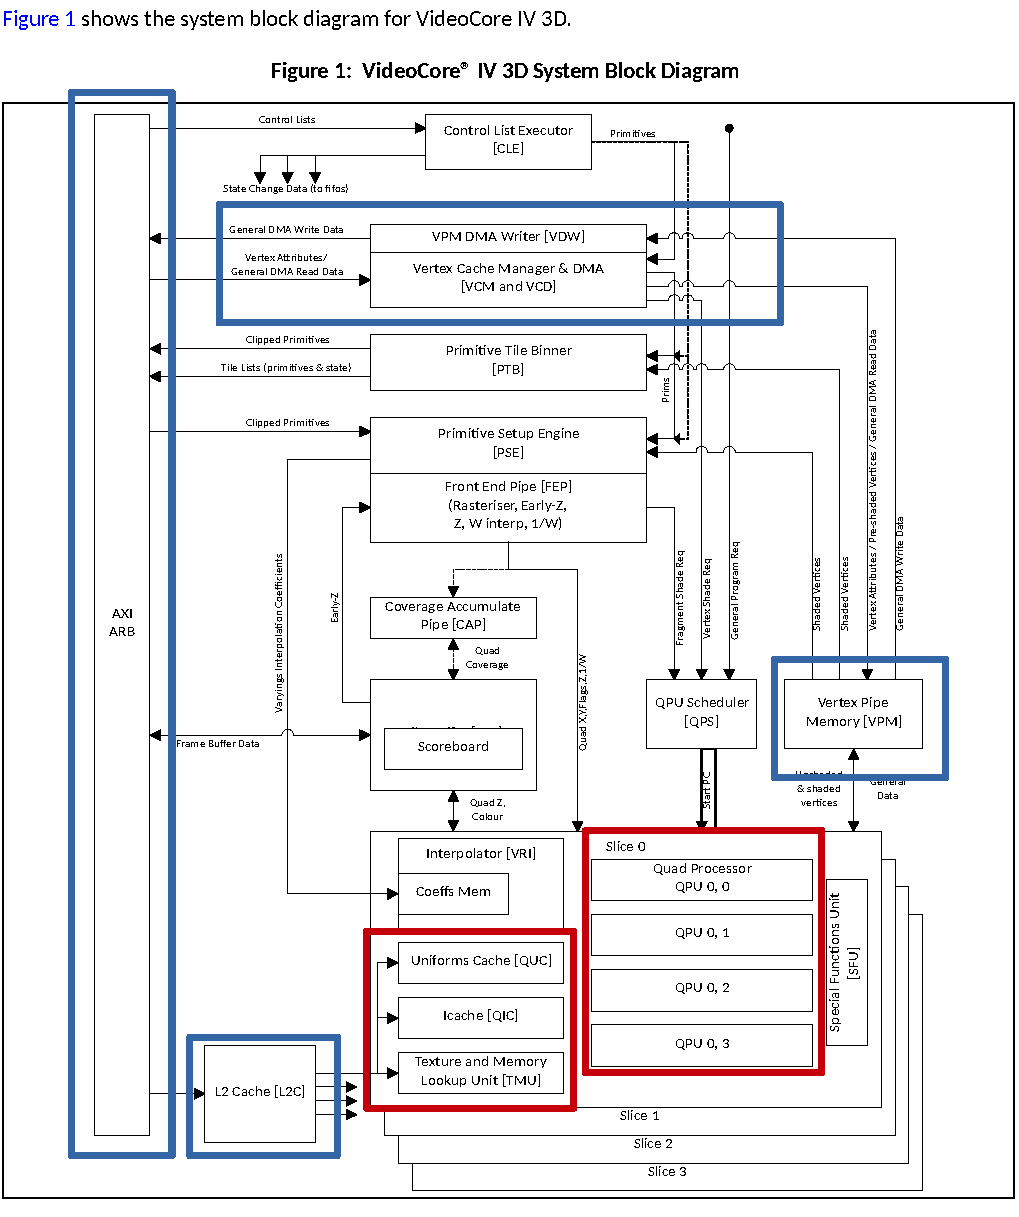
\includegraphics[width=0.9\textwidth]{archOverview}
	\caption{\vc{} archictecture overview}
%\label{sharedFigure}
\end{figure}

% Appendix D

\chapter{\qpu{} pipeline} % Main appendix title

\label{AppendixD} % For referencing this appendix elsewhere, use \ref{AppendixB}

\begin{figure}[!htbp]
	\centering
	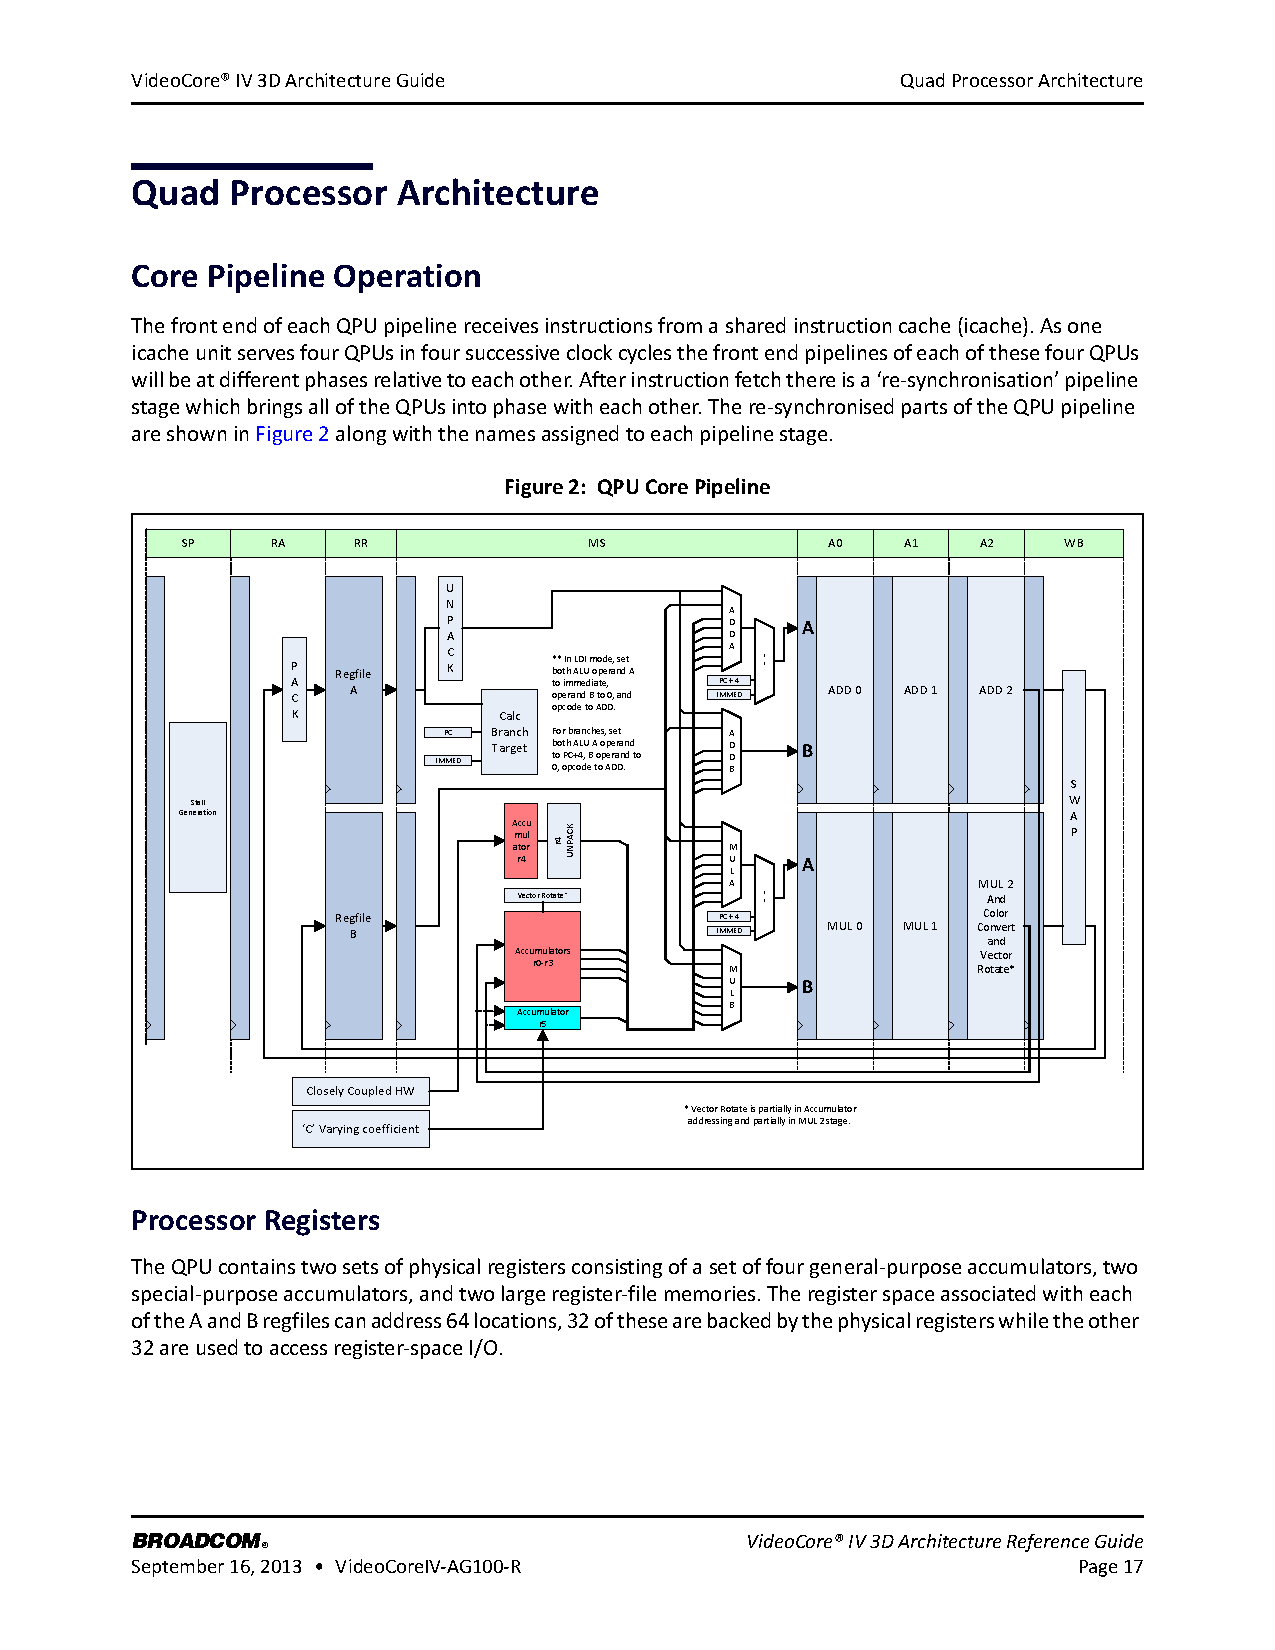
\includegraphics[width=0.9\textwidth]{QPUpipeline}
	%\caption{\qpu{} pipeline}
%\label{sharedFigure}
\end{figure}

% Appendix E

\chapter{\keyword{helloworld} directory} % Main appendix title

\label{AppendixE} % For referencing this appendix elsewhere, use \ref{AppendixB}

\section{\file{driver.c}} % Main appendix title

\lstset{style=CStyle,basicstyle=\tiny,caption={},label=}

\begin{lstlisting}

#include <stdio.h>
#include <stdlib.h>
#include <string.h>
#include <stddef.h>
#include <sys/time.h>

#include "mailbox.h"
#include "qpu.h"

#define NUM_QPUS        1
#define MAX_CODE_SIZE   8192

static unsigned int qpu_code[MAX_CODE_SIZE];



struct memory_map
{
    unsigned int code[MAX_CODE_SIZE];
    unsigned int uniforms[NUM_QPUS][2];     // 2 parameters per QPU
                                            // first address is the input value
                                            // for the program to add to
                                            // second is the address of the
                                            // result buffer
    unsigned int msg[NUM_QPUS][2];
    unsigned int results[NUM_QPUS][16];     // result buffer for the QPU to
                                            // write into
};



int loadShaderCode(const char *fname, unsigned int *buffer, int len)
{
    FILE *in = fopen(fname, "r");
    if (!in)
    {
        fprintf(stderr, "Failed to open %s.\n", fname);
        exit(0);
    }

    size_t items = fread(buffer, sizeof(unsigned int), len, in);
    fclose(in);

    return items;
}



int main(int argc, char **argv)
{
    if (argc < 3)
    {
        fprintf(stderr, "Usage: %s <code .bin> <val>\n", argv[0]);
        return 0;
    }



    int code_words = loadShaderCode(argv[1], qpu_code, MAX_CODE_SIZE);
    printf("Loaded %d bytes of code from %s ...\n", code_words * sizeof(unsigned),
           argv[1]);



    struct GPU_FFT_HOST host;
    if (gpu_fft_get_host_info(&host))
    {
        fprintf(stderr,	"QPU fetch of host information (Rpi version, etc.) failed.\n");

	return -5;
    }



    unsigned uniform_val = atoi(argv[2]);
    printf("Uniform value = %d\n", uniform_val);



    volatile unsigned *peri = (volatile unsigned *) mapmem(host.peri_addr,
                              host.peri_size);
    if (!peri)
    {
        mem_free(mb, handle);
        qpu_enable(mb, 0);
        return -4;
    }



    int mb = mbox_open();
    if (qpu_enable(mb, 1))
    {
        fprintf(stderr, "QPU enable failed.\n");
        return -1;
    }
    printf("QPU enabled.\n");

    unsigned size = 1024 * 1024;
    unsigned handle = mem_alloc(mb, size, 4096, host.mem_flg);
    if (!handle)
    {
        fprintf(stderr, "Unable to allocate %d bytes of GPU memory", size);
        return -2;
    }

    unsigned ptr = mem_lock(mb, handle);



    void *arm_ptr = mapmem(BUS_TO_PHYS(ptr + host.mem_map), size);

    // assert arm_ptr ...
    struct memory_map *arm_map = (struct memory_map *)arm_ptr;
    memset(arm_map, 0x0, sizeof(struct memory_map));

    unsigned vc_uniforms = ptr + offsetof(struct memory_map, uniforms);
    unsigned vc_code = ptr + offsetof(struct memory_map, code);
    unsigned vc_msg = ptr + offsetof(struct memory_map, msg);
    unsigned vc_results = ptr + offsetof(struct memory_map, results);
    memcpy(arm_map->code, qpu_code, code_words * sizeof(unsigned int));



    for (int i = 0; i < NUM_QPUS; i++)
    {
        arm_map->uniforms[i][0] = uniform_val;
        arm_map->uniforms[i][1] = vc_results + i * sizeof(unsigned) * 16;
        arm_map->msg[i][0] = vc_uniforms + i * sizeof(unsigned) * 2;
        arm_map->msg[i][1] = vc_code;
    }

    unsigned ret = execute_qpu(mb, NUM_QPUS, vc_msg, GPU_FFT_NO_FLUSH,
                               GPU_FFT_TIMEOUT);



    // check the results!
    for (int i = 0; i < NUM_QPUS; i++)
    {
        for (int j = 0; j < 16; j++)
        {
            printf("QPU %d, word %d: 0x%08x\n", i, j, arm_map->results[i][j]);
        }
    }



    printf("Cleaning up.\n");
    unmapmem(arm_ptr, size);
    unmapmem((void *)host.peri_addr, host.peri_size);
    mem_unlock(mb, handle);
    mem_free(mb, handle);
    qpu_enable(mb, 0);
    printf("Done.\n");
}

\end{lstlisting}

\newpage

\section{\file{helloworld.asm}} % Main appendix title

%\lstset{style=customasm,basicstyle=\tiny,caption={}}}

\lstinputlisting[caption={}, style=customasm,label=]{helloworld.asm}
%\begin{lstlisting}
%\end{lstlisting}


%----------------------------------------------------------------------------------------
%	BIBLIOGRAPHY
%----------------------------------------------------------------------------------------

\printbibliography[heading=bibintoc]

%----------------------------------------------------------------------------------------

\end{document}
